\documentclass[11pt]{report}
\usepackage[english]{babel}
\usepackage[T1]{fontenc}
\usepackage[utf8]{inputenc}
\usepackage{graphicx}
\usepackage{fancyhdr}
\usepackage{vmargin}									
\usepackage{hyperref}
\usepackage{subfig}
\usepackage{booktabs}
\usepackage{longtable}
\usepackage{wrapfig} % wrap figure around text

% temporary solutions for conditional content, noted as "TMP"
\usepackage{ifthen} 
\newboolean{showOld}
\setboolean{showOld}{true}
%


\setmarginsrb{2.5 cm}{2.5 cm}{2.5 cm}{2.5 cm}{1 cm}{1.5 cm}{1 cm}{1.5 cm}
\graphicspath{{images/}}


\title{Information Systems Security}				        % Title
%\author{Riccardo Zaccone}				            % Author
\author{Marco Smorti \\ Riccardo Zaccone}   % Authors
%\date{\today}										    % Date
\date{January 21, 2021}								    % Date

\makeatletter
\let\thetitle\@title
\let\theauthor\@author
\let\thedate\@date
\makeatother

\hypersetup{
	pdftitle={\thetitle},
	pdfauthor={\theauthor},
	pdfsubject={},
	pdfkeywords={},
	hidelinks}

\pagestyle{fancy}
\fancyhf{}
\lhead{\thetitle}
\cfoot{\thepage}

\begin{document}

%%%%%%%%%%%%%%%%%%%%%%%%%%%%%%%%%%%%%%%%%%%%%%%%%%%%%%%%%%%%%%%%%%%%%%%%%%%%%%%%%%%%%%%%%

\begin{titlepage}
	\centering
	
\includegraphics[scale=0.6]{logoPoli.png}\\[1.0 cm]				
	\textsc{\LARGE POLITECNICO DI TORINO}\\[-0.2 cm]		% Name
	\rule{\linewidth}{0.2 mm} \\
	\textsc{\large Master degree in Computer Engineering}\\[1.0 cm]		
	\rule{\linewidth}{0.2 mm} \\[0.4 cm]
	{ \huge \bfseries \thetitle}\\
	\rule{\linewidth}{0.2 mm} \\%[1 cm]
	\textsc{\Large Notes from the course 01TYMOV of Prof. Antonio Lioy \\ A.A. 2020/21}\\[0 cm]	
	\textsc{}\\[0.4 cm]
	
	\begin{minipage}{0.4\textwidth}
		\begin{flushleft} \large
			\emph{Main authors:}\\
			\theauthor
			\end{flushleft}
			\end{minipage}~
			\begin{minipage}{0.4\textwidth}
			\begin{flushright} \large
		\end{flushright}
	\end{minipage}\\[1.0 cm]



	%DISCLAIMER
	\begin{minipage}{\textwidth}
		IMPORTANT NOTICE: these notes are not in any way promoted or checked by the professor or any
		person of the course teaching staff, so they are provided “AS-IS” and without any guarantee. However,
		we put a great effort to make them and verify their correctness, we hope they will be useful for you.
	\end{minipage}\\ [0.5 cm]

	{\large Version 1.0 \\ \thedate}\\

	
\end{titlepage}


%%%%%%%%%%%%%%%%%%%%%%%%%%%%%%%%%%%%%%%%%%%%%%%%%%%%%%%%%%%%%%%%%%%%%%%%%%%%%%%%%%%%%%%%%
\chapter*{Preliminary notes}
Copyright (C)  2021.

Permission is granted to copy, distribute and/or modify this document
under the terms of the GNU Free Documentation License, Version 1.3
or any later version published by the Free Software Foundation;
with no Invariant Sections, no Front-Cover Texts, and no Back-Cover Texts.
A copy of the license is included in the appendix \ref{appendix:GNU} entitled "GNU
Free Documentation License".
\chapter*{Contributors}

\begin{itemize}
	\item Marco Smorti
	\item Riccardo Zaccone
\end{itemize}
\tableofcontents
\pagebreak

\def\slides{slides/01_intro.pdf}
\chapter{Introduction to the security of ICT systems}


\def\slides{slides/02_crypto_p1.pdf}
\chapter{Cryptographic techniques for cybersecurity}


\section{Cryptography}

\begin{figure}[h]
    \centering
    \includegraphics[page = 2,trim = 0.5cm 3cm 1cm 5cm, clip, width = 0.55\textwidth]{\slides}
\end{figure}


The most used technique to achieve protection for many centuries is \textbf{cryptography}; a mathematical technique that involves algorithms for encryption and decryption:
\begin{itemize}
    \item the encryption algorithm takes a message (in clear) and transforms it in such a way that it becomes unintelligible;
    \item to recover the original text, the decryption algorithms make it readable again.
\end{itemize}
Next to the algorithms, \textbf{key-1} is needed for encryption and \textbf{key-2} for decryption, both of which are streams of bits.
Cryptography is used in communication and for data storage (for example, to store data on disks without permission to read them except for authorized users). The common terminology used in cryptography includes two other keywords:
\begin{itemize}
    \item \textbf{Plaintext} or \textbf{cleartext}: the unencrypted message, typically referred to as \textbf{P};
    \item \textbf{Ciphertext}: the encrypted message, typically referred to as \textbf{C}. Note that in some countries, the term "encrypted" may sound offensive for religious reasons (related to the cult of the dead); in such cases, "\emph{enciphered}" is preferred.
\end{itemize}


\subsection*{Cryptography's strength (Kerchoffs' principle)}
Kerckhoffs' Principle (1883) states that \ul{the security of a cryptosystem must lie in the choice of its keys only};
everything else (including the algorithm itself) should be considered of public knowledge. 
However, this principle relies on the fact that the keys have the following properties.
\begin{itemize}
    \item Are kept \textbf{secret};
    \item Are managed only by \textbf{trusted systems};
    \item Are of \textbf{adequate length} % TODO: cross-reference this
\end{itemize}

If these properties are met, 
not only it has no importance that the encryption and decryption algorithms are kept secret, but it is better to
make the algorithms public so that they can be widely analysed, and their possible flaws and vulnerabilities identified.

\subsection*{Security through obscurity (STO)}
The Kerckhoffs' Principle is related to the concept of \textbf{Security through obscurity}: it means that a system is protected, but the details on how it has been protected are not disclosed.\\
Generally, \ul{this alone is not considered a valid security mechanism} because if someone discovers how the system has been protected (and we have seen that there are also non-technical ways by which this can be achieved), it is no longer secure. 

For this reason, we say that \emph{"Security through obscurity is as bad with computer systems as it is with women"}.
\begin{quote}
    "Men try to hide things from women, but when they discover the truth, it is worse than if they had known it from the beginning"
\end{quote}
\begin{flushright}
    (Antonio Lioy)
  \end{flushright}
\emph{Editor's note:} don't hide things from your partner, regardless of gender.


However, there is a category of people (such as military men) which tend to apply STO, but as an \ul{additional
layer}. It is possible to use STO as a layer only if a really strong algorithm is used (but not a secret one).



\section{Symmetric and asymmetric cryptography}
Depending on which relation exists between key-1 and key-2 there are different kinds of cryptography.

\subsection*{Secret key / symmetric cryptography}
\begin{figure}[h]
    \centering
    \includegraphics[page = 6,trim = 2.5cm 3cm 2.5cm 13cm, clip, width = 0.55\textwidth]{\slides}
\end{figure}

It is so named because \textbf{only a single key} is shared by the sender and receiver. In the diagram, there is a plaintext used as input for the encryption (E) block, along with the key. The result is a comprehensible text that is transmitted to the receiver. To retrieve the original text, the decryption (D) block algorithm is used with the same key that was used for encrypting the initial text. If a different key is used, an output is generated, but it will be incorrect (and typically understandable). 

The issue in the diagram is represented by the dashed line: how can the key be securely shared between the sender and receiver? The formulas used are as follows.

% TODO: fix these formulas 
\begin{align*}
K_1 &= K_2 = K\\
C &= enc(K,P)   & or  C = \{P\} K \\
P &= dec(K,C) = enc^{-1} (K,C)
\end{align*}

\chapter{Authentication techniques and architectures}

\section{What is authentication}


\subsection{Definitions of authentication}
There are three different definitions of \emph{authentication:}
\begin{itemize}
  \item \textbf{RGC-4949 (Internet security glossary)}:\\
        "the process of verifying a claim that a system entity or system
        resource has a certain attribute value"
  \item \textbf{\url{whatis.com}}:\\
        "the process of determining whether someone or something is
        who or what it is declared to be"
  \item \textbf{NIST IR 7298 (Glossary of Key Information Security Terms)}:\\
        "verifying the identity of a user, process, or device, often as a
        prerequisite to allowing access to resources in an information
        system"
\end{itemize}
The key aspects of these definitions  are that they define the authentication of an actor, meaning that \textbf{it could be not only a human being} (interacting via software running on hardware) \textbf{but also a software component or a hardware element} (interacting via software). The common shorthand for authentication is \texttt{authN} or \texttt{authC}, while \texttt{authZ} is used for authorization, \textit{which is different but related}.
% Maybe add a cross-reference to "different but related", idk to what yet


\subsection{Authentication factors}
While authenticating an \emph{actor}, there are three categories of \textbf{authentication factors} that can be used:
\begin{itemize}
  \item \textbf{Knowledge}: authentication relies on something that \emph{only the user knows}, for example a static
        passphrase, code, or personal identification number.\\
        The associated risks involve the storage of this
        knowledge, how it can be demonstrated, and the way it is transmitted.
  \item \textbf{Ownership}: authentication relies on something that \emph{only the user possesses} (often called an
        "authenticator"), for example, a token, smart card, or smartphone.\\
        The associated risks can be related
        to the authenticator itself, such as the possibility of infection with malware, the potential for it to be
        manufactured in a country that imposes government control, or the risk of it being stolen, cloned, or
        used without the owner's authorization (e.g., forgetting an unlocked smartphone).
  \item \textbf{Inherence}: \emph{something the user is}, for example, a biometric characteristic (such as a fingerprint).\\
        The associated risks include counterfeiting and privacy concerns. Inherence factors pose a greater risk
        than the previous cases because, for example, a biometric characteristic \ul{cannot be
          replaced when compromised}. For this reason, inherence factors should be limited to very secure environments,
        typically used only for local authentication, as a mechanism to unlock a secret or a device.
\end{itemize}


\section{Digital authentication model (NIST SP800.63B)}\label{chap:digital-auth-model}

% Image from slide
% \begin{figure}[h]
%   \centering
%   \includegraphics[page = 6,trim = 1cm 2.1cm 1cm 3.8cm, clip, width = 0.50\textwidth]{\slides}
%    \caption{General model for digital authentication as described in NIST SP800.63B}
% \end{figure}

\begin{figure}[h]
  \centering
  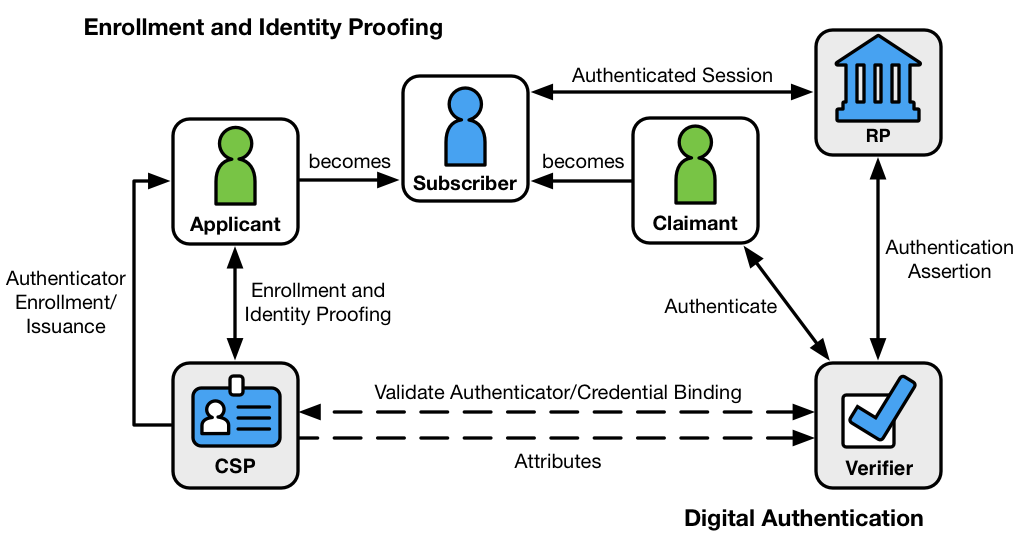
\includegraphics[width = 0.70\textwidth]{chapter3/NIST_sp800_63b.png}
  \caption{General model for digital authentication as described in
    NIST SP800.63B}
\end{figure}

\begin{itemize}
  \item In this model, an actor who wants to use a system
        is called an \colorbox{LimeGreen}{\textbf{applicant}}: if it possesses an
        authenticator it can provide it to the \colorbox{Goldenrod}{\textit{CSP} (Credential Service Provider)}, or it can get one (for example, when a student is enrolled in Politecnico,
        he is given a smart card that works as an
        authenticator). The CSP is that component that will
        issue or enrol user credential and authenticator, and verify and store associated attributes.


        When this procedure is completed successfully, the actor becomes a \colorbox{Cyan}{\textbf{subscriber}}, which is an entity recorded in the authentication system.


  \item Later, when the actor wants to use some network service, typically the actor is called a \colorbox{LimeGreen}{\textbf{claimant}}, because they claim to be a valid user. Typically, an authentication protocol against a \colorbox{Goldenrod}{verifier} is run to verify this claim. When this process ends successfully, the actor becomes
        \colorbox{Cyan}{\textbf{a subscriber}} \textbf{with an open authenticated session} with the \colorbox{Goldenrod}{relying party}, that will request and receive an authN assertion from the Verifier to assess user identity (and attributes).

        The relying party, which requests the actor to be authenticated, is the end application. The verifier may have communication with the CSP to validate the binding between the authenticator used in the authentication protocol and the credential claimed.
\end{itemize}

\subsubsection{Recap}
\begin{itemize}
  \item \textbf{The credential binds an authenticator to the subscriber via an ID}:
        \begin{itemize}
          \item for example, an X.509 certificate can be considered the credential, as it binds the identity and attributes written inside the certificate with the authenticator. In this case, the authenticator is the private key that the user controls.
        \end{itemize}
  \item \textbf{CSP (Credential Service Provider)}:
        \begin{itemize}
          \item will issue or enrol user credential and authenticator
          \item verify and store associated attributes
        \end{itemize}
  \item \textbf{Verifier}:
        \begin{itemize}
          \item executes an authN protocol to verify possess of a valid
                authenticator and credential
        \end{itemize}
  \item \textbf{Relying party}:
        \begin{itemize}
          \item will request/receive an authN assertion from the Verifier to
                assess user identity (and attributes)
        \end{itemize}
\end{itemize}


These roles may be separate or collapsed together.
Thinking about a \emph{Linux machine} used locally, the enrollment phase involves creating a new user with a username (the credential) and a password (the authenticator). In this scenario, the CSP is the operating system itself, and when a user wants to use a server on this machine, they need to perform login, which is the verifier. The relying party is any software running on that machine that uses the identity as proven by the login service of the operating system.



Another example is the use of Google Identity for different services, such as the Doodle Service to schedule an
appointment. For Doodle, there is an option to use Google or Facebook Credentials. In this case, the relying party
is Doodle, while the verifier (as well as the CSP) is Google or Facebook.


\section{Generic authentication protocol}

\begin{figure}[h]
  \centering
  \includegraphics[page = 8,trim = 0.4cm 3cm 0.4cm 5.5cm, clip, width = 0.55\textwidth]{\slides}
  \caption{Generic authentication protocol}
\end{figure}
Suppose that the user wants to access an application server (Relying Party). In this case, the server will include both the Relying Party and Verifier.
The user has been identified with the User ID and has a secret associated with that User ID.
The server's identifier contains a table with the User ID and the result of the function $f$ applied to the secret. Normally, the secret should never be stored in cleartext; of course, if the function $f$ is the identity function, it means you are storing the secret in cleartext, which is not recommended.

When the user wants to access the service, they receive an \textbf{authentication request}. Initially, they provide the \textbf{User ID}, and then the verifier asks for a \textbf{proof request}; the user replies with the \textbf{proof $ = F(S_{\mathrm{UID}})$}, which is the result of the computation with the function $F$ applied to the user's secret.

In this scenario, several problems need to be addressed:
\begin{itemize}
  \item On the user side, how is the secret stored? How is the secret provided (e.g., if it is a password entered via a keyboard, a keylogger could disclose it)? Is the transmission of the proof secure?
  \item On the server side, how are the secrets related to the user stored? When a proof is received, how is it verified to be the correct proof?
\end{itemize}



\subsection{Passwords (reusable)}

\begin{figure}[h]
  \centering
  \includegraphics[page = 9,trim = 0.4cm 5cm 0.4cm 5.5cm, clip, width = 0.55\textwidth]{\slides}
  \caption{Authentication with password}
\end{figure}


Imagine that the secret is a \textbf{reusable password} (meaning that it is always the same), and the user is identified by their User ID, with the secret being the password associated with that user. On the server side, there is a table containing usernames and passwords in plain text or a function $H$ computed over the password.

Once again, there will be an \textbf{authentication request}, followed by the user sending their \textbf{UID}. Then, a password request is made, and the user responds with \textbf{$P_{\text{UID}}$}.

Assume the network is secure and focus on the verifier's side. The secret is the user's password, and the client creates and transmits the proof, typically using a function $F = I$, which is the identity function. The proof is the password sent in plain text, which is, of course, dangerous.

Now, looking at the server, when the server receives the password, it needs to check if it is correct or not:
\begin{enumerate}
  \item first case: if the function $f$ used to store the password is the \textbf{identity function} ($f = I$), then the proof is the password in cleartext. In this scenario, the server knows all the passwords in plain text, and verifying their correctness is simple. However, it is risky; if someone copies the database, they will gain access to all data.
  \item second case (\ul{the suggested one}): $f$ is not the identity function but a \textbf{one-way hash} (a digest of the password), and the server does not know the password in plain text but only the (unprotected) digest $H_{\mathrm{UID}}$. This means that access control is a bit more complex, as when the proof is received, the hash of the proof is computed and compared with the hash stored in the password database. If the database is stolen, the attacker will not have a copy of the plain-text passwords.
\end{enumerate}


\subsubsection{Problems of reusable passwords}
Password-based authentication is usually convenient for the user, but only if they have to remember just one password, a reusable one. The current situation is unfortunate because in some applications, there is a need for several passwords that cannot be remembered by a person, so they would need to be stored on the user's side, which is a source of insecurity. The \textbf{disadvantages} of password-based authentication are:
\begin{itemize}
  \item \textbf{The user-side password storage}: it could be written on a post-it or on a client-side password manager (also called password wallet), that stores it encrypted typically using only one passphrase;
  \item \textbf{Guessable passwords};
  \item \textbf{Server-side password storage}: the server must know the password in cleartext or an unprotected digest of it (dictionary attack);
  \item \textbf{Sniffing}: Password can be sniffed while it is sent across the network;
  \item \textbf{DB attacks}: There could be attacks to the password DB at the verifier (if DB contains plaintext or only obfuscated password);
  \item \textbf{Password guessing}: it is very dangerous if it can be done offline, for example against a list of password hashes;
  \item \textbf{Password enumeration}: if the password is limited in length or character type, or if authN protocol doesn't block;
  \item \textbf{Password duplication}: using the same password for different services, due to user password reuse. This could be a problem because if the user has the same password for a high-security service and for a weaker one, an attacker could discover it on the weaker system and have access to the high-security one;
  \item \textbf{Cryptography aging}: the solution adopted for verifying the secret should not be tied to a specific cryptographic algorithm, because it could be then difficult to adapt to the need for changing the algorithm used, due to new attacks and more computing power;
  \item \textbf{Password capture} via server spoofing and phishing;
  \item \textbf{MITM attacks}.
\end{itemize}



\subsubsection{Password best practice}
\begin{itemize}
  \item Use a \textbf{mixture} of alphabetic characters (both uppercase and lowercase), digits, and special characters. Unfortunately, there are many systems that don't allow the use of special characters or impose limits on password length.
  \item Use a \textbf{long} password, preferably at least 8 characters in length.
  \item \textbf{Avoid using dictionary words}, as attackers often employ dictionaries from multiple languages.
  \item \textbf{Change your password frequently}. If the same password is kept for an extended period, attackers have more time to perform their computations. It's advisable to change your password at least once or twice a year to reduce the window of exposure.
  \item Whenever possible, \textbf{consider not using passwords}. However, this may be unavoidable unless biometric techniques are employed.
\end{itemize}

\subsubsection{Storing passwords}
\paragraph{Storing passwords on the server-side}
\begin{itemize}
  \item Never store passwords in cleartext.
  \item If the password is \textbf{encrypted}, the server must have access to the encryption key in cleartext, which can be a security concern. To enhance security, it's recommended to \textbf{store a password digest}. However, be cautious of dictionary attacks that can be expedited by techniques such as \textbf{rainbow tables}. To mitigate these types of attacks, you can introduce an unpredictable element known as a "\textbf{salt}".
\end{itemize}


\subsubsection{Storing password on the client-side}
\begin{itemize}
  \item Should be only in user's head;
  \item If passwords are a lot, use an encrypted file or a password wallet;
        \ifthenelse{\boolean{showNew}}{
  \item It's better use an encrypted file, or a "password wallet / manager".
        }{}
\end{itemize}

\subsubsection{Storing passwords on the client-side}
\begin{itemize}
  \item Passwords should be memorized by the user.
  \item If there are numerous passwords to manage, consider using an encrypted file or a password wallet.
\end{itemize}



\subsection{The "Dictionary" Attack}
\begin{figure}[h]
  \centering
  
\includegraphics[width = 0.30\textwidth]{chapter3/dictionary_attack.jpg}
\end{figure}

If you store the plain hash of a password, dictionary attacks are possible. This is possible under two hypotheses:
\begin{enumerate}
  \item known hash algorithm;
  \item leakage of information, so that the attacker has a copy of the \textbf{password hash values}.
\end{enumerate}
Hashes are not invertible functions, but it is possible to make a \textbf{pre-computation}. Therefore, even if there is no copy of any password hash yet, it is possible to decide that it would be worthwhile to attack passwords stored as plain SHA-1 hashes in the future.

You must obtain a dictionary containing not only the Italian language but all possible languages.
For each word in the dictionary, you compute the hash of the word and store it in a database paired with the corresponding word.
By "word," we mean a potential passphrase, not a part of it.
Typically, attackers have dictionaries extended to include words such as names of famous people.


The main hypothesis is that the user has chosen one of the words contained in the dictionary. The attack proceeds as follows:
\begin{enumerate}
  \item At some point, the attacker obtains a hash value due to a leakage.
  \item The attacker performs a simple \textbf{lookup} as follows:
        \( w = \mathrm{lookup}(\mathrm{DB}, \mathrm{HP}) \),
        where DB is the database
        and HP is the computed hash of a word in the database, if any of the hash passwords appears in any tuple.
  \item If the response is positive, the password is equal to that word. If not, the password is not from the dictionary.
\end{enumerate}

\textbf{Pre-computation} is the key because if you wait until you get a copy of the password hash, and only at that point you start computing all the possible hash values, it could be too late because the password could have changed.

\subsection{Rainbow table}
A dictionary attack can be made faster and more effective by the \textbf{Rainbow table} technique. It is still a \textit{dictionary attack}, \ul{but it involves a trade-off between space and time}. Trying all possible passwords and computing the hash would be fast, but the result would be a huge database. If you have a complete database, the lookup would be fast, but fewer passwords are stored, and a bit more time is taken to compute the password if the corresponding hash is present. This is an improvement because \ul{it makes an exhaustive attack feasible for certain password sets}.

Imagine creating a rainbow table to attack a password that we know contains 12 digits.
The exhaustive attack would require $10^{12}$ rows, which is a huge number of lines containing passwords and the corresponding hash values.
A rainbow table could be used to reduce the number of rows in the database by a factor of 1000. In this way, we get a $10^9$ rows database, where each line represents 1000 passwords. To achieve that, we use the \textbf{reduction function}:
\[
  r: h \Rightarrow p
\]
It is a function $r$ that takes a hash as input and creates one possible password. \textbf{Beware that this is NOT the inverse of the hash ($h^{-1}$)}, because the inverse of the hash does not exist. It is just a mapping function that, from a hash, creates one of the possible passwords of the whole set; in other words, the reduction function is a different function with a \ul{swapped domain and codomain of the hash function}.

For other informations, check \url{https://en.wikipedia.org/wiki/Rainbow_table}.

\paragraph{Pre-computation}
Then, the pre-computing is the following:

\begin{figure}[h]
  \centering
  \includegraphics[page = 15,trim = 1cm 2.5cm 7cm 13cm, clip, width = 0.55\textwidth]{\slides}
\end{figure}

\begin{enumerate}
  \item Select $10^9$ distinct passwords (the desired size) called $P$.
  \item For each of them, initialize the computation starting from that specific password, and then iterate 1000 times; each time the hash of the current password is computed (called $k$), and then the reduction function is used to go from $k$ to another possible password.
  \item At the end, the password $P$ of the first cycle is stored in the database together with the last computation of the reduction function (called $p$).
  \item Then, the entry implicitly represents all the 1000 passwords tried. Note that there is no more hash to be stored.
\end{enumerate}


\paragraph{Attack}
Then the attack rises in this way:
\begin{figure}[h]
  \centering
  \includegraphics[page = 16,trim = 1cm 8.2cm 3cm 5cm, clip, width = 0.55\textwidth]{\slides}
\end{figure}

\begin{enumerate}
  \item $\mathrm{HP}$ is the leaked hash of a password;
  \item Start an iteration of at most 1000 times, and each time, the reduction function is used to derive a possible password from the hash value;
  \item Next, search the database to check if there is a row where $p$ (the result of the reduction function) is at the end of the chain. In that case, we found the chain containing that hash; otherwise, a new value $k$ is calculated by performing the password hash;
  \item After finding the chain, the computation of the hash must be done again to identify which hash matches the one we have.
\end{enumerate}

The problem is that since the reduction function is going from a hash to one possible password, there could be
two different hashes that generates the same password, and this is called \textbf{fusion}. Rather than using a reduction
function, a set of n reduction functions is used, one for each reduction step. On internet there are on sale pre-
computed rainbow tables for various hash functions and password sets (e.g., SHA1 for alphanumeric).


This technique is used by various attack programs.


\subsection{Using salt in storing passwords}
The critical point in the previous kind of attack is that the attacker performs pre-computation. Without the rainbow
table and without the database created by the dictionary,
it would take a lot of time. For this reason, \textbf{do not provide the attacker with the information needed for pre-computation},
because it is based on the idea that the attacker may know which is the password (through the dictionary).

\begin{itemize}
  \item Using the following technique, even if it can be possible to guess what a possible password is, the attacker
        does not get the hash table because every time a User ID is created, the system generates a \textbf{salt} that is different for each user.\\
        The salt is a random (unpredictable) and long (increased dictionary complexity) string of bytes.
        Users do not have to memorize the salt, which should contain rarely used or control characters.\\
        Then the hash is computed using the password concatenated with salt:\\
        $\mathrm{HP} = hash(pwd | salt)$;
  \item The verifier stores UID,
        $\mathrm{HP}_{\mathrm{UID}}$ and $salt_{\mathrm{UID}}$.\\
        If someone gets the information in the database, he also gets the salt, but only then the
        computation can start, which will require a lot of time and in the meanwhile the password could have been
        changed. Additionally, there are different HP for users having the same password.
\end{itemize}

This makes the dictionary attacks nearly impossible (including those based on rainbow tables).


\subsubsection{Example: Passwords in Linux}
Originally stored in \texttt{/etc/passwd}, hashed with a DES-based
hash function named \texttt{crypt()}.
Since \texttt{/etc/passwd} needs to be world-readable (contains
usernames, UID, GID, home, shell, etc.), passwords have been
moved to \texttt{/etc/shadow}, readable only by system processes.
Passwords are stored in the following form - see \texttt{crypt(5)}:

\begin{verbatim}
  $id$salt$hashedpwd
\end{verbatim}
Different hash functions are used depending on the ID, for example:
\begin{itemize}
  \item 1 = MD5, \ldots, 5 = SHA-256, 6 = SHA-512, \ldots
\end{itemize}
If \texttt{\$id\$salt} is absent, the old DES-based hash is used (with
a 12-bit salt, and the password is truncated to 8 characters) - danger!
Some algorithms have adjustable complexity (to counter brute-force attacks).


\begin{casehistory}{The LinkedIn Attack}
  In June 2012, someone was able to copy 6.5 million passwords from LinkedIn, which were unsalted plain SHA-1
  hashes. The person published those hashes on the internet and asked for crowdsourcing, used for cooperative
  password cracking (which means trying to compute SHA-1 hashing of words and looking if someone has a match).
  At least 236,578 passwords were found before Interpol was able to ban the website that published the
  password hashes.

  Note that simultaneously LinkedIn found out that the LinkedIn app for iPad/iPhone was sending in clear sensitive data
  (not relevant to LinkedIn!).
\end{casehistory}

\subsubsection{Example: Passwords in MySQL}
\textbf{MySQL} is a database where usernames and passwords are stored in the "user" table. MySQL (from v4.1) uses a \textbf{double hash (without salt!)} to store passwords:
\[
  \texttt{SHA-1(SHA-1(password))}
\]
Then, the hex encoding of the result is stored, preceded by * (to distinguish this case from MySQL versions < 4.1). For example, for the password "Superman!!!," the field \texttt{user.password} is
\begin{verbatim}
    user.password = *868E8E4F0E782EAA610A67B01E63EF04817F60005
\end{verbatim}
To verify that this is the double hash of the word, you can use the following command on Linux:
\begin{verbatim}
  $ echo -n "Superman!!!" | sha1sum | xxd -r -p | sha1sum
\end{verbatim}
This is the standard way for MySQL to store passwords, which is not secure. It is advisable to change the standard way MySQL uses to store passwords by using a salted approach.


\section{Strong (peer) authN}
Recently, there has been a growing emphasis on the requirement to move away from standard authentication methods and adopt strong peer authentication. While this is consistently requested in specifications, it is often not formally defined or defined in multiple, potentially confusing ways.



\subsection{ECB Definition for Internet Banking}
According to the European Central Bank (ECB), \ul{strong customer authentication (authN) is a procedure based on the use of two or more of knowledge, ownership, and inherence.} The selected elements must be \ul{mutually independent}, ensuring that the breach of one does not compromise the others. At least one element should be non-reusable and non-replicable (except for inherence), and not capable of being surreptitiously stolen via the Internet. The strong authentication procedure should be designed to protect the confidentiality of the authentication data; for example, if a password is used, it cannot be sent in clear text.



\subsection{PCI-DSS definition for payment with credit cards}
According to PCI-DSS definition, which is for payment with credit cards, starting from v3.2 it requires multi-
factor authentication (MFA) for access into the cardholder data environment (CDE): it does not matter if it
a trusted or untrusted network, and it is also used when the access is performed by administrators. The only
exception is with direct console access (physical security), which means that you enter the room where the server is placed. For remote access it is always required from untrusted network and by users and third-parties (such as maintenance).
This was the best practise until Jan '18 and it has been made compulsory afterwards.
\textbf{Remember}: MFA is \textbf{not} twice the same factor (e.g., two passwords).


\subsection{PCI-DSS Definition for Payment with Credit Cards}
According to the PCI-DSS definition, which applies to payment with credit cards, starting from v3.2, multi-factor authentication (MFA) is required for access into the cardholder data environment (CDE). This requirement is applicable regardless of whether the network is trusted or untrusted, and it is also mandatory for administrators accessing the CDE.

The only exception is for direct console access, which involves physical security measures, such as entering the room where the server is located. However, for remote access, MFA is always required, especially from untrusted networks, and for users and third parties (e.g., maintenance).

This best practice was in effect until January '18 and became mandatory thereafter.

\textbf{Remember}: MFA does \textbf{not} mean using the same factor twice, like using two passwords.



\subsection{Other definitions}
According to the \textit{Handbook of Applied Cryptography},\\
authentication is a \textbf{cryptographic challenge-response identification protocol}.

More in general, it is a technique resisting to a well-defined set of attacks.

An authN technique can be classified as strong or weak depending on the attack model:
\begin{itemize}
  \item E.g., users of Internet Banking follow the ECB definition;
  \item E.g., employees of PSP adhere to the PCI-DSS definition.
\end{itemize}

In general, pay attention to your specific application field because it defines the types of risks and the level of strength required for your strong authentication.




\section{Challenge-Response Authentication (CRA)}
Challenge-response protocol is a possible way to implement strong authentication. CRA means that there is a
challenge sent to the Claimant from the Verifier. The Claimant replies with the solution computed using some
secret knowledge and the challenge. The Verifier compares the response with a solution computed via a secret
associated with the Claimant.


% Using minipage
\vspace{2mm}
\noindent
\begin{minipage}{0.5\textwidth}
  \centering
  \includegraphics[page = 25,trim = 0.5cm 2.2cm 1cm 9.8cm, clip, width = \linewidth]{\slides}
\end{minipage}
\hspace{0.05\textwidth}
\begin{minipage}{0.4\textwidth}
  Someone claims to own the identifier (ID). The verifier looks that there is a row
  associated with that ID and sends to the
  claimant the challenge. The claimant has
  a key (\(K_c\)) and uses it to perform some
  kind of computation (function \(f\)) and
  generates a response. The response can
  be checked by applying the function \(g\) to
  the challenge and to a well-known key (\(K_V\)) of the Verifier. The keys can be different or the same.
\end{minipage}


\subsubsection{General issues of CRA}
\begin{itemize}
  \item \textbf{The challenge must be non-repeatable to avoid replay attacks}. For this reason, usually, the challenge
        is a (random) nonce.
  \item \textbf{The function \(f\) must be non-invertible}, otherwise, a listener can record the traffic and easily find the
        shared secret by using the function \(K_c = f^{-1}(response, challenge)\).
\end{itemize}



\subsection{Symmetric CRA}

\noindent
\begin{minipage}{0.5\textwidth}
  \centering
  \includegraphics[page = 27,trim = 0.5cm 2.2cm 1cm 9.8cm, clip, width = \linewidth]{\slides}
\end{minipage}
\hspace{0.05\textwidth}
\begin{minipage}{0.4\textwidth}
  In this case, there is a common key
  shared between Claimant and Verifier,
  which is typically the password or
  passphrase of the user. The function \(f\) is computed two times: once from the user
  to make the response, and once from the
  verifier to verify the match.
\end{minipage}

\subsubsection{General issues of Symmetric CRA}
General issues with Symmetric CRA are:
\begin{itemize}
  \item The easiest implementation uses a hash function (faster than encryption) such as SHA1 (deprecated),
        SHA2 (recommended) or SHA3 (future);
  \item \(K_{ID}\) must be known in cleartext to the Verifier and this may lead to attacks against the \( \{ID: K_{ID}\} \) table at the Verifier;
\end{itemize}
There is a technique called \textbf{SCRAM} (Salted CRA Mechanism) which solves this problem by using hashed
passwords at the Verifier, which also offers \underline{channel binding} and \underline{mutual authentication}, while we are always talking about single authentication


\subsubsection{Mutual symmetric CRA (v1)}
\noindent
\begin{minipage}{0.4\textwidth}
  Imagine that we are not using a hash but encryption (although it would work in the same way), and let's consider the scenario of mutual authentication.

  Alice and Bob share a key \(K_{AB}\), and Alice sends a message \(A\) to Bob (which means: "Hey, I'm Alice!").
  Bob responds with a challenge \(C_B\),
  and Alice replies with \(\text{enc}(K_{AB}, C_B)\), which is the encryption of the challenge using the shared key.
  Then, Alice could create a challenge (\(C_A\)), and Bob would respond in the same way by computing \(\text{enc}(K_{AB}, C_A)\).
  \ul{This approach provides protection against MITM attacks because, if the challenges are nonces, the Replay Attack is not possible.}

  \textbf{Beware!} This protocol is outdated and insecure.
\end{minipage}
\hspace{0.05\textwidth}
\begin{minipage}{0.5\textwidth}
  \centering
  \includegraphics[page = 29,trim = 4cm 2.2cm 4cm 9cm, clip, width = \linewidth]{\slides}
\end{minipage}

\subsubsection{Mutual symmetric CRA (v2)}
\vspace*{5mm}
\noindent
\begin{minipage}{0.4\textwidth}
  IBM, in its SNA network system, employed a similar technique with a different implementation: they reduced the number of messages for improved performance without compromising security.

  In the initial step, Alice transmits both the identity (\(A\)) and the challenge (\(C_A\)). The response from Bob includes both the challenge (\(C_B\)) and the encryption \(\text{enc}(K_{AB}, C_A)\). Finally, Alice responds with \(\text{enc}(K_{AB}, C_B)\). Although this may appear equivalent to the previous solution in terms of functionality and security, \underline{it is not}.

\end{minipage}
\hspace{0.05\textwidth}
\begin{minipage}{0.5\textwidth}
  \centering
  \includegraphics[page = 30,trim = 4cm 2.2cm 4cm 9cm, clip, width = \linewidth]{\slides}
\end{minipage}




\subsubsection{Attack to the mutual symmetric CRA (v2)}
\vspace*{5mm}
\noindent
\begin{minipage}{0.4\textwidth}
  Here, Mike pretends to be Alice. Mike sends to Bob Alice's identity (\(A\)) and Alice's challenge (\(C_A\)). Bob replies with \(C_B\) and \(\text{enc}(K_{AB}, C_A)\).

  At this point, Mike does not know \(K_{AB}\) and cannot compute the response to the challenge. However, Mike opens a new connection with Bob, sending Alice's identity (\(A\)) again but, this time, sends the challenge sent from Bob (\(C_B\)). Bob replies again with another challenge (\(C_C\)) and \(\text{enc}(K_{AB}, C_B)\), which is the answer to the challenge of the 1st connection. Mike can finally provide the correct answer.

  \ul{Of course, this can be countered if there is a limit on connections}.
\end{minipage}
\hspace{0.05\textwidth}
\begin{minipage}{0.5\textwidth}
  \centering
  \includegraphics[page = 31,trim = 2cm 2.2cm 2cm 4cm, clip, width = \linewidth]{\slides}
\end{minipage}

\ifthenelse{\boolean{showNew}}{
  \subsubsection{GSM (in)security}
  In our discussion on improved authentication methods beyond basic passwords, we highlighted the effectiveness of the challenge-response approach with symmetric keys. To illustrate this concept in a real-world scenario, let's delve into GSM authentication and its relevance to security.


  \textbf{GSM} (\textit{Global System for Mobile Communications}) has been designed violating the principle of security through obscurity and
  relies on three confidential algorithms:
  \begin{itemize}
    \item A8, operating within the \underline{SIM} (Subscriber Identity Module), focuses on symmetric key generation, laying the foundation for secure connections.
    \item A3, also embedded in the \underline{SIM}, handles authentication processes, providing a robust framework for verifying user identities.
    \item Additionally, A5, a stream cipher implemented in the \underline{mobile device}, contributes to data encryption, safeguarding sensitive information during transmission.
          \begin{itemize}
            \item GSM's security approach introduces some level of secrecy through the implementation of A5/1 and A5/2, where A5/1 is the more commonly used variant and A5/2 is intentionally weakened in specific regions for surveillance purposes.
            \item A5/3, based on the Kasumi block cipher, offers an alternative encryption method, but it's not widely used.
          \end{itemize}
  \end{itemize}

  Implementing \textbf{security through obscurity}, as highlighted, is inherently problematic. This approach is not only detrimental in terms of the algorithm's efficacy but also raises concerns about the design process itself. The fact that a limited group of individuals crafted the process without seeking revisions, reviews, or insights from external experts resulted in a suboptimal design. This underlines the importance of inclusive and collaborative design practices for creating robust and effective security measures.

  Furthermore, the discretion of Mobile Network Operators (MNOs) comes into play, allowing them to choose algorithms for A8, A3, and A5. Typically, A8 and A3 are constructed using the COMP128 secret function, involving the computation of \[Z = \text{COMP128}(X, Y)\]
  with each variable being 128 bits.
  A8 extracts the least significant 54 bits of Z to generate the connection key \[Kc = lsb( 54, Z )\]
  while A3 utilizes the most significant 32 bits of Z to produce a "\textit{Signed RESponse}" \[SRES = msb( 32, Z )\]
  actually this is not a digital signal because it is not using any public key.

  \paragraph{GSM Security Overview}
  \begin{figure}[h]
    \centering
    \includegraphics[page = 34,trim = 3cm 3cm 3cm 4cm, clip, width = 0.50\textwidth]{\slides}
    \caption{GMS authentication}
  \end{figure}
  \begin{figure}[h]
    \centering
    \includegraphics[page = 35,trim = 3cm 3cm 3cm 4cm, clip, width = 0.50\textwidth]{\slides}
    \caption{GMS encryption}
  \end{figure}
  In GSM authentication, a symmetric Challenge-Response Authentication (CRA) is employed to verify the identity of the Mobile Station (\textbf{MS}),such as a mobile phone, to the Base Station (\textbf{BS}) through its SIM.
  The SIM holds an \textbf{individual subscriber authentication key} ($Ki$), a confidential 128-bit secret shared with the Authentication Centre (AC). \\
  The process unfolds as the BS transmits a random 128-bit challenge ($C$) to the SIM, and in response, the SIM computes the 32-bit Signed Response (SRES) using the A3 algorithm with inputs $C$ and $Ki$:
  \[\text{SRES} = A3( C, Ki )\]
  This value is, in fact, a keyed digest, as it is computed based on a key.


  However, a notable vulnerability arises with COMP128-1, which is identified as weak. Exploiting chosen-challenge and differential cryptanalysis techniques, a relatively modest number of challenges, around 150,000, are adequate to compute Ki. This weakness opens the door to potential security breaches, enabling actions such as SIM cloning, where an unauthorized party can replicate the SIM, sharing the same Ki.\\
  Consequently, with the compromised Ki, the attacker gains the ability to decrypt the communication traffic by computing the Connection Key ($Kc$) for that specific Ki and the challenge ($C$) sent by the BS. This vulnerability highlights the importance of addressing weaknesses in authentication protocols to ensure the integrity of GSM security.
}{}


\subsection{Asymmetric CRA}
\begin{figure}[h]
  \centering
  \includegraphics[page = 36,trim = 0.5cm 2.3cm 0.5cm 8cm, clip, width = 0.55\textwidth]{\slides}
  \caption{Asymmetric CRA}
\end{figure}
It is also possible to employ an asymmetric challenge-response mechanism. In this scenario, the user does not transmit their identity directly but rather provides their X.509 certificate, which declares both their identity and public key (the claimant possesses the corresponding private key, $ID.PK$). The Verifier initiates the process by generating a challenge, employing a random nonce \(R\) encrypted with the public key. The claimant decrypts the challenge using their private key and returns the decrypted value to the Verifier. If the response matches the \(R\) value specified in the challenge, it confirms possession of the private key. The only necessary verification involves checking if a valid ID is registered in the Verifier's database.

\paragraph{Asymmetric CRA: analysis}
Asymmetric Challenge-Response Authentication (CRA) is \ul{the strongest usable mechanism}, eliminating the need for storing any secrets at the Verifier. It is consistently implemented for \textit{peer authentication} (client and server) in protocols such as IPsec, SSH, and TLS. Additionally, it serves as a fundamental component for user authentication in a new authentication system named FIDO (Chapter \href{chap:fido}).
% TODO: cross-reference FIDO

However, it comes with certain downsides:
\begin{itemize}
  \item \textbf{Slowness}, stemming from the inherent sluggishness of asymmetric cryptography.
  \item Inaccurate design may result in \textbf{unintentional signature creation by the Claimant}.
        The Claimant, while receiving something, performs a computation with the private key.
        This computation, used both for decryption and creating a signature, poses a risk of inadvertently signing a document. To mitigate this risk, the data provided as input for decryption on the claimant-side must follow a \underline{specific format}.
  \item Public Key Infrastructure (\textbf{PKI}) \textbf{issues}, including concerns related to \textit{trusted roots}, \textit{name constraints}, and \textit{revocation}, since it relies on certificates. These issues can be avoided if the Verifier stores \(ID.PK\), however this strategy shifts the equivalent PKI effort to the Verifier.
        This approach is adopted by SSH, wherein the public key is taken and made public on the server, despite with the significant risk of someone potentially altering the key stored on the server.
\end{itemize}


\subsection{One-time password (OTP)}
\begin{figure}[h]
  \centering
  \includegraphics[page = 38,trim = 0.5cm 3cm 1cm 5cm, clip, width = 0.55\textwidth]{\slides}
  \caption{One Time Password (OTP)}
\end{figure}
Instead of employing reusable passwords, users are assigned passwords that are valid for a single login session. When a claimant seeks access to the server, they respond by providing their userID. Subsequently, the server issues a request for a specific password from an extensive list, for instance, password number 48. If passwords $P49_{UID}$ and $P50_{UID}$ have already been utilized, the user transmits $P48_{UID}$ and marks it as used in the table.

At this juncture, the server maintains a table containing user identifiers (UID) and the undisclosed secret ($S_{UID}$) that the user is unaware of.
This secret is utilized for password generation. The Verifier, in turn, replicates the function used to generate the password to regenerate it and verifies if it aligns with the one transmitted by the user. This methodology renders passwords \textbf{immune to} potential \textbf{sniffing attacks}, as they can be transmitted in plaintext, knowing that the subsequent login will involve a different password.

\paragraph{Summary}
\begin{itemize}
  \item The password in this authentication protocol is \textbf{only valid for a single run}, necessitating a new password for each subsequent authentication session.
  \item This characteristic makes it \textbf{immune to sniffing attacks}, as the intercepted password becomes obsolete after one use.
  \item However, it is \textbf{subject to} Man-in-the-Middle (\textbf{MITM}) attacks when an entity assumes the role of the verifier. To mitigate this risk, Verifier authentication is essential.
  \item Provisioning for subscribers involves managing a large number of passwords, leading to potential password exhaustion.
  \item Additionally, \textbf{inserting passwords can be challenging} due to their typically random and complex nature, designed to prevent guessing attacks.
\end{itemize}

\subparagraph{OTP provisioning to the users}
For OTP provisioning to users, additional precautions may be necessary when the claimant operates on a device lacking computational capabilities or on an insecure/untrusted workstation. In such cases, physical safety measures can include:
\begin{itemize}
  \item A sheet of paper containing pre-computed passwords.
  \item Hardware authenticator (crypto token): a device where passwords are stored or generated.
\end{itemize}

By contrast, when working on an intelligent and secure/trusted workstation, OTPs can be \textbf{automatically computed} by a dedicated application (commonly found in smartphones, tablets, laptops, etc.).


\subsubsection{The S/KEY system}
This was the first OTP definition and implementation by Bell Labs (1981).
\begin{itemize}
  \item The user generates a secret \(S_{ID}\).
  \item Then the user autonomously computes \(N\) one-time passwords where \(P_1 = h(S_{ID})\), \(P_2 = h(P_1)\), ..., \(P_N = h(P_{N-1})\) (associated hash).
  \item The Verifier stores the last one \(P_N\). This password will never be used directly for authentication but only indirectly.
  \item When the user wants to access the server, the Verifier (which has \(P_N\)) asks for \(P_{N-1}\) and gets \(X\) from the user. Then the following check is performed:
        % TODO: align them as with code
        \begin{align*}
          \text{if } (P_N \neq h(X)) \text{ then FAIL} \\
          \text{else OK; store } X \text{ as } P_{N-1}
        \end{align*}
\end{itemize}



\begin{figure}[h]
  \centering
  \includegraphics[page = 43,trim = .5cm 2.1cm .5cm 3.6cm, clip, width = 0.55\textwidth]{\slides}
  \caption{The S/KEY System}
\end{figure}


The technique employed here involves the Verifier requesting passwords \textbf{in reverse order}. This approach allows the Verifier to operate without the need to possess knowledge of the user's secret, placing the responsibility on the user to be familiar with all passwords. This methodology is detailed in RFC-1760 and employs MD4 (although alternative options are possible). \(S/KEY\) serves as an illustration of an Off-line / Pre-computed OTP.

It is crucial to note that \textbf{MITM} (Man-in-the-Middle) \textbf{attacks are possible with OTP}. Consequently, \(S/KEY\) should be utilized in conjunction with \textbf{server authentication}.


\paragraph{S/KEY - generation of the password list}
The user inserts a passphrase (PP), which must be a minimum of 8 characters long and kept secret. If disclosed, the security of S/KEY is compromised. The passphrase is concatenated with a server-provided seed (sent in cleartext from S to C), allowing the use of the same passphrase for multiple servers (using different seeds). It is also possible to safely reuse the same passphrase by changing the seed.

A 64-bit quantity is extracted from the MD4 hash, which generates a 128-bit result (by XORing the first/third 32-bit groups and the second/fourth groups).

\paragraph{S/KEY - passwords}
64-bit passwords represent a compromise, and entering them in hexadecimal form requires 16 characters. Typically, they are input as a sequence of six short English words selected from a dictionary of 2048 (e.g., 0 = A, 1 = ABE, 2 = ACE, 3 = ACT, 4 = AD, 5 = ADA).

This entails choosing 11 bits from the computed hash and utilizing a dictionary with simple words corresponding to the combinations (2048 in this case). \textbf{It is crucial that the client and server share the same dictionary}. For instance:
\begin{itemize}
  \item \textbf{Password (text)}: "YOU SING A NICE OLD SONG," not because it serves as a password but because “YOU” is one of the words in the dictionary, representing 11 bits. In total, there are 6 words, resulting in 66 bits (more than 64, ensuring security).
  \item \textbf{Password (numeric)}: 1D6E5001884BD711 (hex) or 2,120,720,442,049,943,313 (decimal).
\end{itemize}
This is merely an illustrative example of encoding a lengthy bit string in a user-friendly manner.


\subsubsection{Time-based OTP}
\begin{figure}[h]
  \centering
  \includegraphics[page = 46,trim = 1cm 3cm 1cm 7cm, clip, width = 0.55\textwidth]{\slides}
  \caption{Time Based OTP}
\end{figure}
In this solution, the password depends on time and the user's secret:
\[p(ID, t) = h(t, S_{ID})\]
When the claimant wants to authenticate, it receives a request from the verifier and submits its own ID plus the value generated by a device (authenticator), which tells the claimant which is the correct password to be entered at that moment. At that point, the verifier needs to check if the value is the current OTP for the current time. Since the verifier has a large table containing, for each user, the corresponding secret, it can perform the same computation and compare it.

This type of OTP requires local computation at the subscriber and clock synchronization (or keeping track of time-shift for each subscriber). Due to the fact that the password needs time to be sent, the time needs to be quantized (considering timeslots, usually ranging from 30 to 60 seconds), and an authentication window is established. Usually, the verifier considers the password as correct if it is generated one timeslot before or one timeslot after the correct timeslot according to its own time. In formulas, the authentication succeeds if\footnote{Here "$\Vert$" means \texttt{logical or} instead of \texttt{concatenated}}
\[
  X == p(ID, t) \quad \Vert \quad
  X == p(ID, t - 1)
  \quad \Vert \quad X == p(ID, t + 1)
\]
(where \(t\) is the timeslot). Typically, only one authentication run per timeslot is allowed, which might not be suitable for some services, for example, a broker that needs to perform many transactions concurrently.

This system is \textbf{susceptible to time-based attacks} against both subscribers and the Verifier. Typically, servers and clients synchronize their time with an external source, and \ul{an attack can be executed using a fake NTP server or a mobile network femtocell}. For instance, if an attacker successfully deceives the subscriber into providing a password for a future timeslot, they can exploit it at that specific time.

Since the Verifier stores the secret for each user, it must manage a highly sensitive database. In the event of a security breach where the database is compromised, the attacker gains the ability to impersonate users and compute the passwords for any user. An incident of this nature occurred in an attack against a TOTP system named \textit{RSA SecurID}.

\paragraph{A TOTP example: RSA SecurID}
In this system, the Claimant sends the triple \{\textit{user},\textit{PIN}, \textit{tokencode(seed, time)}\} in clear to the Verifier.
As \textit{RSA SecurID} is a physical device continuously displaying the correct password, if someone other than the subscriber reads and uses it, an attacker could gain access with the subscriber's identity. This emphasizes the need for an additional authentication factor. Therefore, one factor is "\textit{owning the device}" while the other is "\textit{knowing the (reusable) password}".

Since it could be possible for the PIN to be sniffed while sent across the network, there is a variant of the \textit{SecurID} authenticator that includes a “pin pad” (a sort of small keyboard just for entering the PIN).
When the PIN is entered, the value of the PIN is taken into account for the generation of the OTP. In this case, it is possible to send just the user and the modified token code (the tuple \{\textit{user, token-code*(seed, time, PIN)}\}), which is also a function of the PIN.
Based on the user and PIN, the Verifier checks against three possible token codes: $TC_{-1}$, $TC_{0}$, $TC_{+1}$, as in any TOTP system.

\begin{figure}[h]
  \centering
  \includegraphics[page = 49,trim = .5cm 2.05cm .5cm 4cm, clip, width = 0.55\textwidth]{\slides}
\end{figure}
Moreover, each device is associated with \underline{two PINs}: the first one is the one used normally for \underline{authentication}, while the second is called \underline{duress code}, and it is used to generate an alarm when the subscriber is under attack (for example, when the user is forced by a criminal to authenticate).


\subparagraph{SecurID: architecture}
\begin{figure}[h]
  \centering
  \includegraphics[page = 50,trim = .5cm 2.2cm .5cm 4cm, clip, width = 0.55\textwidth]{\slides}
  \caption{SecurID: architecture}
  \label{fig:ace}
\end{figure}

Besides providing the hardware authenticator which computes the token code,
RSA also provides some component called \textbf{ACE} (Access Control Engine):
\begin{itemize}
  \item \textbf{ACE client} is installed at the Relying Party, which is the server that wants to use the authentication system;
  \item \textbf{ACE server} implements the Verifier.
\end{itemize}
In the illustration (Figure \ref{fig:ace}), the ACE server positioned at the top serves as the verifier, possessing the comprehensive information required to validate a token code. The service servers represent the Relying Party, entities necessitating access control integration with RSA SecurID. To interact with the verifier and authenticate user credentials, these servers must implement the ACE client. On the left of the depicted scenario, remote access to an SSH server is illustrated: the user, equipped with a standard SecurID device, submits the triple \texttt{\{user, PIN, TC\}}. Upon receiving this information, the Relying Party forwards it to the verifier, which subsequently delivers a response indicating the validity of the provided credentials. On the right side of the picture, an unsuccessful authentication attempt is exemplified, employing a device with a pin pad.

The significance of examining this architecture extends beyond its role as a SecurID implementation. It serves as a comprehensive model, highlighting the need for server enhancements to accommodate specialized authentication methods (e.g., DBMS software in the provided example). When a company aims to deploy a uniform authentication technology across various servers, a centralized verifier becomes essential. This verifier can offer authentication verification services for all relaying parties, drawing parallels with the \textit{NIST schema} (Chapter \ref{chap:digital-auth-model}) in this regard.



\subsubsection{Event-based OTP}
The principal problem with TOTP is that only one authentication per timeslot is allowed.
This solution introduces a monotonic integer counter, denoted as $C$, as an additional input alongside the seed:
\[
  p(ID, C) = h(C, S_{ID})
\]

It requires local computation at the subscriber, where the counter is incremented (e.g., through a button press), allowing for frequent authentication runs.
While this system enables OTP pre-computation, even by adversaries with temporary access to the authenticator, it poses challenges for the Verifier in handling \textbf{desynchronization} issues. For instance, if the subscriber unintentionally triggers the button, desynchronization may occur.
To address this, a counter window is considered, defining a set of counters with a fixed and typically small size. In formula terms, a password is deemed correct if
\[
  X == p(ID, C) || X == p(ID, C + 1) || X == p(ID, C + 2) || \ldots
\]
with a maximum of ten subsequent counters to resist exhaustive attacks.
\ul{Verifiers can adapt to desynchronization, storing the counter that matched the password sent by the user}.
If none of the passwords generated on the user side is acceptable, a counter reset may be required, such as in cases where a child presses the button more than ten times.


\subsubsection{Out-of-band OTP}
\begin{figure}[h]
  \centering
  \includegraphics[page = 52,trim = 1cm 3cm 1cm 5cm, clip, width = 0.55\textwidth]{\slides}
  \caption{Out-of-band OTP}
\end{figure}

The solutions illustrated so far require the user to receive something: a list of passwords in the case of S/KEY or a device in the case of TOTP and EOTP. In situations where these options are not feasible, such as the inability to securely provide the list or a lack of trust in the user's device, Out-of-Band OTP can be utilized. This method is based on generating the OTP without using the normal communication channel.

In the schema depicted in the figure, the user is provided with a secret key, which is a \textit{reusable password}. During authentication, the user sends the user ID and the reusable password, necessary for clear user identification. Although reusable passwords may not be very robust, the verifier can ensure the user's authenticity through the third step: it looks up the registered phone number in its database. Subsequently, the verifier generates an OTP and sends it (out of band) to the user's cell phone, typically via SMS (step four). This process is considered out of band because the OTP transmission uses a different medium than the communication between the server and the user. Finally, in step five, the user provides the OTP just received.

% TODO: is this good practice?
\paragraph{}
This is a widely used system by many banks and identity providers, such as those involved in SPID. This system also reduces the burden on the user, who does not need to have a modern smartphone but just a minimal device to receive the message: the OTP is generated by the server only when needed and then sent in a trusted way to the user. However, be aware that at step five, a secure channel with server authentication is needed to avoid MITM attacks. The Out-of-Band (OOB) channel is frequently a text via SMS message. Since most mobile networks are nowadays implemented with VoIP, mobile user identification, and SS7 protocol (which are quite insecure), NIST suggests using the Push mechanism over a TLS channel to the registered subscriber device. This is done by putting the message inside a notification, the confirmation of which is made by inserting the user's fingerprint.


\subsubsection{Two-/Multi- Factors AuthN (2FA/MFA)}
It has already been pointed out that, if we want to provide strong authentication, more than one factor should be used. This is also named \textbf{2FA}, or more generally, \textbf{MFA}. MFA is used both to increase authentication strength and to protect the physical authenticator, as seen with OTP. Usually, a \textbf{PIN} is used for authenticator protection.
\begin{itemize}
  \item \textbf{PIN transmitted along with OTP:} As seen, the possible problem is that it can be sniffed when entered or transmitted across the network.
  \item \textbf{PIN entered to compute the OTP itself:} Like in RSA SecurID.
  \item \textbf{PIN (or inherence factor) used to unlock the authenticator,} which is very risky if:
        \begin{itemize}
          \item No protection from \textbf{multiple unlock attempts}.
          \item \textbf{The lock mechanism} is weak, for example, the fingerprint sensor is not strong enough to recognize only the device owner's fingerprint.
          \item \textbf{Unlocking is valid for a time window}: if someone has access to the authenticator in the time window in which it is unlocked, then they can use the user identity.
        \end{itemize}
\end{itemize}

\subparagraph{Importance of MFA: the Iphone ransomware}
In May 2014, a security incident occurred involving iCloud accounts with single-factor authentication, resulting in unauthorized access.
The attackers employed a "remote lock" feature through the "Find My Device" functionality. Users of affected devices, such as iPhones and iPads, received a menacing message indicating the breach: "\textit{Device hacked by Oleg Pliss!}"
The attackers demanded a payment of 100 USD/EUR via a specified PayPal account (lock404(at)hotmail.com) for the restoration of control.

Alternatively, users were informed of the option to use "recovery mode," although this came at the cost of losing all device data and applications. It's crucial to note that even complying with the payment demand did not guarantee a resolution, as the attackers provided a fake PayPal account.
This incident highlighted the vulnerabilities associated with single-factor authentication and emphasized the importance of robust security measures in safeguarding user accounts.\\
\href{http://thehackernews.com/2014/05/apple-devices-hacked-by-oleg-pliss-held.html}{More info here.}

\subsection{Authentication of human beings}
Ensuring that the subscriber is a human rather than a program can be achieved through two solutions:
\begin{itemize}
  \item \textbf{CAPTCHA} techniques (\textit{Completely Automated Public Turing test to tell Computers and Humans
          Apart}): for example, a picture with images of distorted characters;
  \item \textbf{Biometric} techniques: for example, fingerprints.
\end{itemize}


\subsubsection{Biometric systems}
The main idea is to measure a biological characteristic of the user, such as fingerprint, voice, retinal scan, iris scan, hand's blood vein pattern, heart rate, and hand geometry.
EHowever, it is important to note that each technique can potentially be circumvented. Moreover, biometrics is not replaceable, highlighting the necessity of implementing additional security measures to mitigate potential vulnerabilities.
Regardless of the chosen biometric solution, two parameters must be considered:

\begin{figure}[h]
  \centering
  \includegraphics[page = 59,trim = 2.5cm 2.5cm 2.5cm 4cm, clip, width = 0.55\textwidth]{\slides}
  \caption{FAR and FRR}
\end{figure}

\begin{itemize}
  \item \textbf{FAR (False Acceptance Rate):} the rate at which the system incorrectly accepts a biometric signal as valid.
  \item \textbf{FRR (False Rejection Rate):} the rate at which the system erroneously rejects a valid signal as if it were fake.
\end{itemize}
The two normal distributions refer to fingerprints that match (green) and those that do not. The two distributions overlap, necessitating the establishment of a threshold. Regardless of where the threshold is set, it is important to note that FAR and FRR cannot both be equal to zero.
They may be partly tuned, but they heavily depend on the cost of the device. Moreover, some biological characteristics are variable; for example, the user can have a finger wound, the voice altered due to emotion, or retinal blood pattern altered due to alcohol or drugs.

Other than technical challenges, there are also various non-technical issues:
\begin{itemize}
  \item \textbf{Psychological acceptance}:
        \begin{itemize}
          \item "Big Brother" syndrome, related to personal data collection.
          \item Some technologies are intrusive and could be harmful; for example, retinal scans may not be suitable for everyone.
        \end{itemize}
  \item \textbf{Privacy concerns} arise since, at this point, it is not just a matter of authentication but of identification, making it irrepudiable.
  \item Biometric features \textbf{cannot be changed} if copied. Unlike passwords, which can be changed if there is a fear of disclosure, a biometric authentication cannot. Therefore, it should not be sent across the network and can only be useful for locally replacing a PIN or a password.
  \item \textbf{Lack of a standard API/SPI} leads to:
        \begin{itemize}
          \item High development costs.
          \item Heavy dependence on single/few vendors.
        \end{itemize}
\end{itemize}

%\ifthenelse{\boolean{showNew}}{
\subsection{Kerberos (and SSO)}

Kerberos, named after the three-headed dog from Greek mythology that guarded the entrance to the underworld, is an authentication system based on a \textit{Trusted Third Party} (\textbf{TTP}).
Originally developed as part of the MIT project Athena, Kerberos holds significance beyond the realm of HTTP-based services.

One of its distinguishing features is its innovative approach to user password management; rather than transmitting passwords across the network, Kerberos utilizes them \underline{only locally}, as \textbf{symmetric cryptographic keys}.
In the Kerberos framework, there are two important concepts:
\begin{itemize}
  \item the term "\textbf{realm}" denotes the Kerberos domain, which represents the collection of systems employing Kerberos as their authentication system.
  \item Additionally, a \textbf{credential} within Kerberos is identified as \texttt{user.instance@realm}, resembling an email address but specific to the Kerberos domain. This structure attaches to each user the role that the user is assuming at this moment for a given operation.
\end{itemize}


\paragraph{Ticket}
Kerberos employs a data structure known as a \underline{ticket} for client authentication to servers. These tickets possess a \textbf{variable lifetime}. In the earlier Version 4, the maximum duration was restricted to 21 hours, structured around five-minute time slots, totaling 255. However, in the more recent Version 5, the validity period is explicitly defined, allowing tickets to be valid for an extended duration, even years. Despite being potentially unlimited, it is recommended to opt for shorter duration tickets to mitigate potential security risks associated with prolonged authentication privileges.

One notable characteristic of Kerberos tickets is their encryption with the \textbf{symmetric key of the target server}. This encryption ensures that the ticket remains secure and can only be decrypted at the destination server, adding an extra layer of protection to the authentication process.

In the initial Kerberos \textit{Version 4}, \textbf{tickets were bound to the IP address of the client}, serving as an identifier for accessing a specific server. However, recognizing the vulnerability of IP addresses to spoofing, this association with IP addresses was eliminated in Version 5, enhancing the robustness of the Kerberos authentication system.

It's essential to highlight that each ticket is uniquely tied to a single credential. If a user possesses multiple credentials, they must obtain distinct tickets for each credential. While the primary purpose of tickets is to facilitate client authentication, Kerberos also offers the optional feature of server authentication using these tickets.

% \begin{figure}[h]
%   \centering
%   \includegraphics[page = 63,trim = 1cm 2.5cm 1cm 4cm, clip, width = 0.55\textwidth]{\slides}
%   \caption{Kerberos High-level view}
% \end{figure}


\subsubsection{Protocol description}
The protocol is described in detail below\footnote{Editor's note: This section is taken from \url{https://en.wikipedia.org/wiki/Kerberos_(protocol)}. I thought it could be simpler and more concise, and it aligns with the content in the slides}.
See Figure \ref{fig:kerberos}.

\begin{figure}[H]
  \centering
  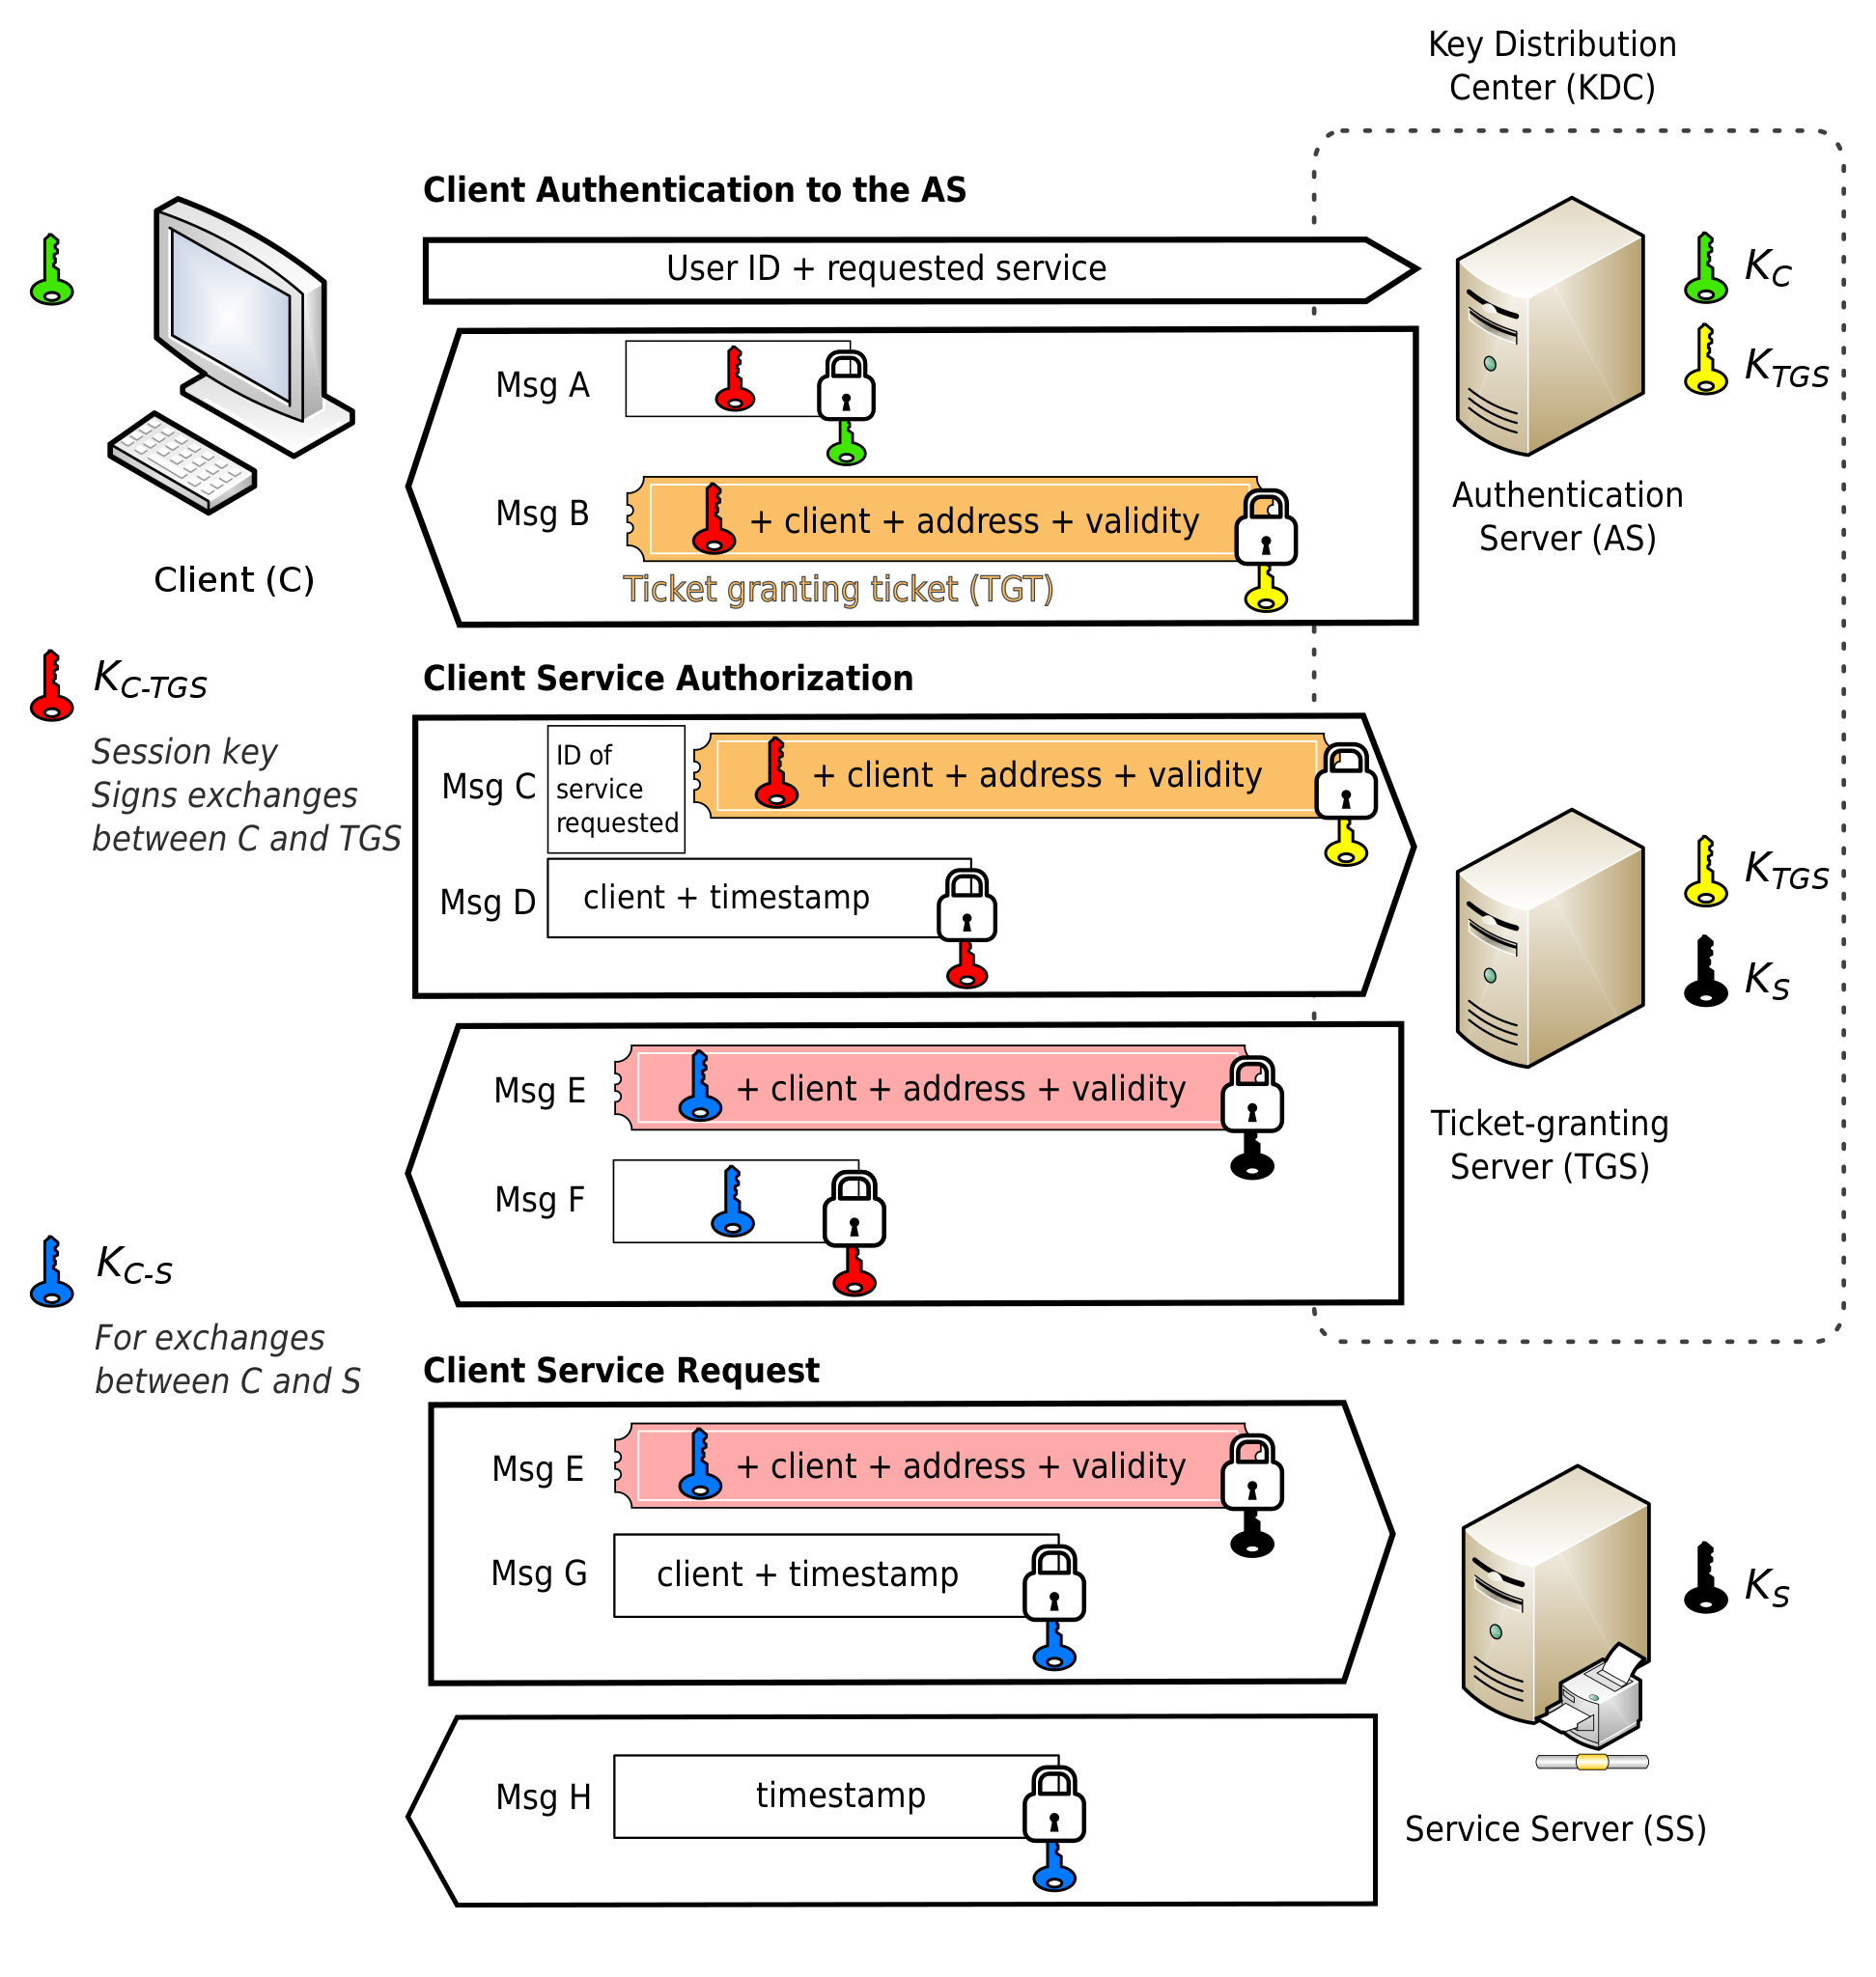
\includegraphics[trim = 1cm 1cm 1cm 1cm, clip, width = 0.9\textwidth]{chapter3/kerberos.png}
  \caption{Kerberos protocol}
  \label{fig:kerberos}
\end{figure}

% TODO This is just for comparison, consider removing it
\paragraph*{User Client-based Login example without Kerberos}

\begin{enumerate}
  \item A user enters a username and password on the client machine(s). Other credential mechanisms like pkinit (RFC 4556) allow for the use of public keys in place of a password. The client transforms the password into the key of a symmetric cipher. This either uses the built-in key scheduling, or a one-way hash, depending on the cipher-suite used.
  \item The server receives the username and symmetric cipher and compares it with the data from the database. Login was a success if the cipher matches the cipher that is stored for the user.
\end{enumerate}


\paragraph*{Client Authentication}

\begin{enumerate}
  \item The client sends a cleartext message of the user ID to the AS (Authentication Server) requesting services on behalf of the user. (Note: Neither the secret key nor the password is sent to the AS.)
  \item The AS checks to see whether the client is in its database. If it is, the AS generates the secret key by hashing the password of the user found at the database (e.g., Active Directory in Windows Server) and sends back the following two messages to the client:
        \begin{itemize}
          \item Message A: \texttt{Client/TGS Session Key} encrypted using the secret key of the client/user.
          \item Message B: \texttt{Ticket-Granting-Ticket} (TGT, which includes the client ID, client network address, ticket validity period, and the \texttt{Client/TGS Session K}ey) encrypted using the secret key of the TGS.
        \end{itemize}
  \item Once the client receives messages A and B, it attempts to decrypt message A with the secret key generated from the password entered by the user. If the user entered password does not match the password in the AS database, the client's secret key will be different and thus unable to decrypt message A. With a valid password and secret key, the client decrypts message A to obtain the \texttt{Client/TGS Session Key}. This session key is used for further communications with the TGS. (Note: The client cannot decrypt Message B, as it is encrypted using TGS's secret key.) At this point, the client has enough information to authenticate itself to the TGS.
\end{enumerate}



\paragraph*{Client Service Authorization}
\begin{enumerate}
  \item When requesting services, the client sends the following messages to the TGS:
        \begin{itemize}
          \item Message C: Composed of the message B (the encrypted TGT using the TGS session key) and the ID of the requested service.
          \item Message D: Authenticator (which is composed of the client ID and the timestamp), encrypted using the \texttt{Client/TGS Session Key} (found by the client in Message A).
        \end{itemize}
  \item Upon receiving messages C and D, the TGS retrieves message B out of message C. It decrypts message B using the TGS secret key. This gives it the Client/TGS Session Key and the client ID (both are in the TGT). Using this \texttt{Client/TGS Session Key}, the TGS decrypts message D (Authenticator) and compares the client IDs from messages B and D; if they match, the server sends the following two messages to the client:

        \begin{itemize}
          \item Message E: \texttt{Client-to-server ticket} (which includes the client ID, client network address, validity period, and Client/Server Session Key) encrypted using the service's secret key.
          \item Message F: \texttt{Client/Server Session Key} encrypted with the \texttt{Client/TGS Session Key}.
        \end{itemize}
\end{enumerate}



\paragraph*{Client Service Request}

\begin{enumerate}
  \item Upon receiving messages E and F from TGS, the client has enough information to authenticate itself to the Service Server (SS). The client connects to the SS and sends the following two messages:

        \begin{itemize}
          \item Message E: From the previous step (the \texttt{Client-to-server ticket}, encrypted using service's Secret key by the TGS).
          \item Message G: A new Authenticator, which includes the client ID, timestamp and is encrypted using \texttt{Client/Server Session Key}.
        \end{itemize}

  \item  The SS decrypts the ticket (message E) using its own secret key to retrieve the \texttt{Client/Server Session Key}. Using the sessions key, SS decrypts the Authenticator and compares client ID from messages E and G; if they match server sends the following message to the client to confirm its true identity and willingness to serve the client:

        \begin{itemize}
          \item Message H: The timestamp found in client's Authenticator (plus 1 in version 4, but not necessary in version 5), encrypted using the \texttt{Client/Server Session Key}.
        \end{itemize}

  \item The client decrypts the confirmation (message H) using the \texttt{Client/Server Session Key} and checks whether the timestamp is correct. If so, then the client can trust the server and can start issuing service requests to the server.
  \item The server provides the requested services to the client.
\end{enumerate}


\paragraph*{Kerberos versions}
Kerberos has evolved through various versions, with MIT V4 marking its original implementation. The subsequent version, MIT V5 (also known as RFC-1510), introduced significant enhancements.
Unlike its predecessor, MIT V5 supports encryption beyond DES, offering increased security options. Notably, it extended the ticket lifetime by specifying explicit begin-end validity periods.
Additionally, MIT V5 introduced features such as inter-realm authentication, forwardable tickets, and extendable tickets. This version enabled users to achieve a single login for access to all Kerberized services. These services encompassed a diverse range, including K-POP, K-NFS, K-LPD, K-telnet, K-ftp, and K-dbms.
Furthermore, Kerberos found adoption in Windows domains, with Microsoft incorporating it into their systems starting from Windows 2000.

The subsequent evolution of Kerberos is reflected in \texttt{RFC-4120}, which supersedes \texttt{RFC-1510}. One notable improvement is the introduction of algorithm flexibility, allowing clients and servers to support different encryption algorithms. Originally, Kerberos utilized DES-CRC32, but over time, it expanded its repertoire to include 3DES, RC4, AES, Camellia, MD4, and MD5.

To enhance security, \texttt{RFC-4120} introduced pre-authentication measures, aiming to thwart password enumeration or dictionary attacks on the Ticket Granting Ticket (TGT). For instance, in Windows, the \texttt{AS\_REQ} must contain encrypted forms of the user's key and timestamp.

\paragraph*{TGT request with PKINIT}
\texttt{RFC-4120} (v5) brings support for asymmetric cryptography, applicable specifically in the \texttt{AS\_REQ} phase, the initial phase of the protocol when making a request to the authentication server.


This feature, known as \texttt{PKINIT} (Public Key Initialization), modifies the Ticket Granting Ticket (TGT) request. In this process, a user seeks a ticket for the Ticket Granting Server (TGS). Unlike previous versions, the authentication server no longer stores user passwords, significantly improving security. Even in the event of an attack on the authentication server, no clear passwords are compromised. Instead, the server stores the public keys of users. Consequently, the server's response to the user's request is encrypted not with a password but with the user's public key. To decrypt this response, the user employs their private key, eliminating the need for storing passwords. In essence, the user relies on a key pair—public and private—rather than a password, and the authentication server utilizes the public key for encryption in the initial step of the authentication process. This paradigm shift represents a substantial advancement in security and authentication within the Kerberos framework.


\begin{figure}[H]
  \centering
  \begin{subfigure}{0.45\textwidth}
    \includegraphics[page=65, trim=.7cm 4cm .7cm 5cm, clip, width=\textwidth]{\slides}
    \caption{TGT request}
  \end{subfigure}
  \hfill
  \begin{subfigure}{0.45\textwidth}
    \includegraphics[page=70, trim=.7cm 4cm .7cm 5cm, clip, width=\textwidth]{\slides}
    \caption{TGT request with PKINIT}
  \end{subfigure}
  \caption{Client authentication}
\end{figure}



\subsubsection*{SSO (Single Sign-On)}

Kerberos is an example of a more general concept of \textit{SSO} (Single Sign-On), where users possess a single "credential" to authenticate themselves and gain access to various services in the system. 

\begin{itemize}
  \item \textbf{Fictitious SSO:}
        \begin{itemize}
          \item Client for automatic password synchronization/management (alias "password wallet").
          \item Specific for some applications only.
        \end{itemize}

  \item \textbf{Integral SSO:}
        \begin{itemize}
          \item Multi-application authentication techniques (e.g., asymmetric CRA, Kerberos), likely requiring a change in the applications.
          \item Multi-domain SSO (e.g., with SAML tokens, that generalize Kerberos tickets).
        \end{itemize}
\end{itemize}



\subsection{Authentication interoperability}

\begin{figure}[h]
  \centering
  \includegraphics[page = 72,trim = 1cm 2.5cm 1cm 10cm, clip, width = 0.55\textwidth]{\slides}
\end{figure}

As mentioned, companies that manage numerous servers aim to implement a unified authentication system for all their relying parties, namely the application servers. However, this implies the ability to purchase a verifier and use it with devices created by different companies. In the past, achieving such interoperability was challenging. For instance, when acquiring RSA SecurID devices, it was necessary to also procure the ACE client and ACE server from RSA. Moreover, RSA did not disclose the hash algorithm used in generating the token code.

To address this challenge, an initiative called \href{http://www.openauthentication.org/}{OATH} was introduced. The primary goal of OATH is to establish \ul{interoperability among authentication systems based on One-Time Passwords (OTPs) and symmetric or asymmetric challenges}. This is achieved through the development of standards for the client-server protocol and the data format on the client, aiming to realize universal strong authentication.

So far, OATH has provided the following specifications:
\begin{itemize}
    \item HOTP (HMAC OTP, RFC-4226)
    \item TOTP (Time-based OTP, RFC-6238)
    \item OATH Challenge-Response Protocol (OCRA, RFC-6287)
    \item Portable Symmetric Key Container (PSKC, RFC-6030): When using OTP, the shared secret must be protected. This solution offers an XML-based key container for transporting symmetric keys and key-related metadata.
    \item Dynamic Symmetric Key Provisioning Protocol (DSKPP, RFC-6063): It is a client-server protocol for provisioning symmetric keys to a crypto-engine by a key-provisioning server.
\end{itemize}

\chapter{Security of IP networks}

\chapter{Security of network applications}
\chapter{Firewall and IDS/ISP}
\chapter{E-mail security}



\appendix
%\pagenumbering{arabic}

\hfuzz = .6pt % avoid black boxes

\chapter{\rlap{GNU Free Documentation License}}
\phantomsection  % so hyperref creates bookmarks
\addcontentsline{toc}{chapter}{GNU Free Documentation License}
\label{appendix:GNU}

\begin{center}
	
	Version 1.3, 3 November 2008
	
	
	Copyright \copyright{} 2000, 2001, 2002, 2007, 2008  Free Software Foundation, Inc.
	
	\bigskip
	
	\texttt{<https://fsf.org/>}
	
	\bigskip
	
	Everyone is permitted to copy and distribute verbatim copies
	of this license document, but changing it is not allowed.
\end{center}


\begin{center}
	{\bf\large Preamble}
\end{center}

The purpose of this License is to make a manual, textbook, or other
functional and useful document ``free'' in the sense of freedom: to
assure everyone the effective freedom to copy and redistribute it,
with or without modifying it, either commercially or noncommercially.
Secondarily, this License preserves for the author and publisher a way
to get credit for their work, while not being considered responsible
for modifications made by others.

This License is a kind of ``copyleft'', which means that derivative
works of the document must themselves be free in the same sense.  It
complements the GNU General Public License, which is a copyleft
license designed for free software.

We have designed this License in order to use it for manuals for free
software, because free software needs free documentation: a free
program should come with manuals providing the same freedoms that the
software does.  But this License is not limited to software manuals;
it can be used for any textual work, regardless of subject matter or
whether it is published as a printed book.  We recommend this License
principally for works whose purpose is instruction or reference.


\begin{center}
	{\Large\bf 1. APPLICABILITY AND DEFINITIONS\par}
	\phantomsection
	\addcontentsline{toc}{section}{1. APPLICABILITY AND DEFINITIONS}
\end{center}

This License applies to any manual or other work, in any medium, that
contains a notice placed by the copyright holder saying it can be
distributed under the terms of this License.  Such a notice grants a
world-wide, royalty-free license, unlimited in duration, to use that
work under the conditions stated herein.  The ``\textbf{Document}'', below,
refers to any such manual or work.  Any member of the public is a
licensee, and is addressed as ``\textbf{you}''.  You accept the license if you
copy, modify or distribute the work in a way requiring permission
under copyright law.

A ``\textbf{Modified Version}'' of the Document means any work containing the
Document or a portion of it, either copied verbatim, or with
modifications and/or translated into another language.

A ``\textbf{Secondary Section}'' is a named appendix or a front-matter section of
the Document that deals exclusively with the relationship of the
publishers or authors of the Document to the Document's overall subject
(or to related matters) and contains nothing that could fall directly
within that overall subject.  (Thus, if the Document is in part a
textbook of mathematics, a Secondary Section may not explain any
mathematics.)  The relationship could be a matter of historical
connection with the subject or with related matters, or of legal,
commercial, philosophical, ethical or political position regarding
them.

The ``\textbf{Invariant Sections}'' are certain Secondary Sections whose titles
are designated, as being those of Invariant Sections, in the notice
that says that the Document is released under this License.  If a
section does not fit the above definition of Secondary then it is not
allowed to be designated as Invariant.  The Document may contain zero
Invariant Sections.  If the Document does not identify any Invariant
Sections then there are none.

The ``\textbf{Cover Texts}'' are certain short passages of text that are listed,
as Front-Cover Texts or Back-Cover Texts, in the notice that says that
the Document is released under this License.  A Front-Cover Text may
be at most 5 words, and a Back-Cover Text may be at most 25 words.

A ``\textbf{Transparent}'' copy of the Document means a machine-readable copy,
represented in a format whose specification is available to the
general public, that is suitable for revising the document
straightforwardly with generic text editors or (for images composed of
pixels) generic paint programs or (for drawings) some widely available
drawing editor, and that is suitable for input to text formatters or
for automatic translation to a variety of formats suitable for input
to text formatters.  A copy made in an otherwise Transparent file
format whose markup, or absence of markup, has been arranged to thwart
or discourage subsequent modification by readers is not Transparent.
An image format is not Transparent if used for any substantial amount
of text.  A copy that is not ``Transparent'' is called ``\textbf{Opaque}''.

Examples of suitable formats for Transparent copies include plain
ASCII without markup, Texinfo input format, LaTeX input format, SGML
or XML using a publicly available DTD, and standard-conforming simple
HTML, PostScript or PDF designed for human modification.  Examples of
transparent image formats include PNG, XCF and JPG.  Opaque formats
include proprietary formats that can be read and edited only by
proprietary word processors, SGML or XML for which the DTD and/or
processing tools are not generally available, and the
machine-generated HTML, PostScript or PDF produced by some word
processors for output purposes only.

The ``\textbf{Title Page}'' means, for a printed book, the title page itself,
plus such following pages as are needed to hold, legibly, the material
this License requires to appear in the title page.  For works in
formats which do not have any title page as such, ``Title Page'' means
the text near the most prominent appearance of the work's title,
preceding the beginning of the body of the text.

The ``\textbf{publisher}'' means any person or entity that distributes
copies of the Document to the public.

A section ``\textbf{Entitled XYZ}'' means a named subunit of the Document whose
title either is precisely XYZ or contains XYZ in parentheses following
text that translates XYZ in another language.  (Here XYZ stands for a
specific section name mentioned below, such as ``\textbf{Acknowledgements}'',
``\textbf{Dedications}'', ``\textbf{Endorsements}'', or ``\textbf{History}''.)  
To ``\textbf{Preserve the Title}''
of such a section when you modify the Document means that it remains a
section ``Entitled XYZ'' according to this definition.

The Document may include Warranty Disclaimers next to the notice which
states that this License applies to the Document.  These Warranty
Disclaimers are considered to be included by reference in this
License, but only as regards disclaiming warranties: any other
implication that these Warranty Disclaimers may have is void and has
no effect on the meaning of this License.


\begin{center}
	{\Large\bf 2. VERBATIM COPYING\par}
	\phantomsection
	\addcontentsline{toc}{section}{2. VERBATIM COPYING}
\end{center}

You may copy and distribute the Document in any medium, either
commercially or noncommercially, provided that this License, the
copyright notices, and the license notice saying this License applies
to the Document are reproduced in all copies, and that you add no other
conditions whatsoever to those of this License.  You may not use
technical measures to obstruct or control the reading or further
copying of the copies you make or distribute.  However, you may accept
compensation in exchange for copies.  If you distribute a large enough
number of copies you must also follow the conditions in section~3.

You may also lend copies, under the same conditions stated above, and
you may publicly display copies.


\begin{center}
	{\Large\bf 3. COPYING IN QUANTITY\par}
	\phantomsection
	\addcontentsline{toc}{section}{3. COPYING IN QUANTITY}
\end{center}


If you publish printed copies (or copies in media that commonly have
printed covers) of the Document, numbering more than 100, and the
Document's license notice requires Cover Texts, you must enclose the
copies in covers that carry, clearly and legibly, all these Cover
Texts: Front-Cover Texts on the front cover, and Back-Cover Texts on
the back cover.  Both covers must also clearly and legibly identify
you as the publisher of these copies.  The front cover must present
the full title with all words of the title equally prominent and
visible.  You may add other material on the covers in addition.
Copying with changes limited to the covers, as long as they preserve
the title of the Document and satisfy these conditions, can be treated
as verbatim copying in other respects.

If the required texts for either cover are too voluminous to fit
legibly, you should put the first ones listed (as many as fit
reasonably) on the actual cover, and continue the rest onto adjacent
pages.

If you publish or distribute Opaque copies of the Document numbering
more than 100, you must either include a machine-readable Transparent
copy along with each Opaque copy, or state in or with each Opaque copy
a computer-network location from which the general network-using
public has access to download using public-standard network protocols
a complete Transparent copy of the Document, free of added material.
If you use the latter option, you must take reasonably prudent steps,
when you begin distribution of Opaque copies in quantity, to ensure
that this Transparent copy will remain thus accessible at the stated
location until at least one year after the last time you distribute an
Opaque copy (directly or through your agents or retailers) of that
edition to the public.

It is requested, but not required, that you contact the authors of the
Document well before redistributing any large number of copies, to give
them a chance to provide you with an updated version of the Document.


\begin{center}
	{\Large\bf 4. MODIFICATIONS\par}
	\phantomsection
	\addcontentsline{toc}{section}{4. MODIFICATIONS}
\end{center}

You may copy and distribute a Modified Version of the Document under
the conditions of sections 2 and 3 above, provided that you release
the Modified Version under precisely this License, with the Modified
Version filling the role of the Document, thus licensing distribution
and modification of the Modified Version to whoever possesses a copy
of it.  In addition, you must do these things in the Modified Version:

\begin{itemize}
	\item[A.] 
	Use in the Title Page (and on the covers, if any) a title distinct
	from that of the Document, and from those of previous versions
	(which should, if there were any, be listed in the History section
	of the Document).  You may use the same title as a previous version
	if the original publisher of that version gives permission.
	
	\item[B.]
	List on the Title Page, as authors, one or more persons or entities
	responsible for authorship of the modifications in the Modified
	Version, together with at least five of the principal authors of the
	Document (all of its principal authors, if it has fewer than five),
	unless they release you from this requirement.
	
	\item[C.]
	State on the Title page the name of the publisher of the
	Modified Version, as the publisher.
	
	\item[D.]
	Preserve all the copyright notices of the Document.
	
	\item[E.]
	Add an appropriate copyright notice for your modifications
	adjacent to the other copyright notices.
	
	\item[F.]
	Include, immediately after the copyright notices, a license notice
	giving the public permission to use the Modified Version under the
	terms of this License, in the form shown in the Addendum below.
	
	\item[G.]
	Preserve in that license notice the full lists of Invariant Sections
	and required Cover Texts given in the Document's license notice.
	
	\item[H.]
	Include an unaltered copy of this License.
	
	\item[I.]
	Preserve the section Entitled ``History'', Preserve its Title, and add
	to it an item stating at least the title, year, new authors, and
	publisher of the Modified Version as given on the Title Page.  If
	there is no section Entitled ``History'' in the Document, create one
	stating the title, year, authors, and publisher of the Document as
	given on its Title Page, then add an item describing the Modified
	Version as stated in the previous sentence.
	
	\item[J.]
	Preserve the network location, if any, given in the Document for
	public access to a Transparent copy of the Document, and likewise
	the network locations given in the Document for previous versions
	it was based on.  These may be placed in the ``History'' section.
	You may omit a network location for a work that was published at
	least four years before the Document itself, or if the original
	publisher of the version it refers to gives permission.
	
	\item[K.]
	For any section Entitled ``Acknowledgements'' or ``Dedications'',
	Preserve the Title of the section, and preserve in the section all
	the substance and tone of each of the contributor acknowledgements
	and/or dedications given therein.
	
	\item[L.]
	Preserve all the Invariant Sections of the Document,
	unaltered in their text and in their titles.  Section numbers
	or the equivalent are not considered part of the section titles.
	
	\item[M.]
	Delete any section Entitled ``Endorsements''.  Such a section
	may not be included in the Modified Version.
	
	\item[N.]
	Do not retitle any existing section to be Entitled ``Endorsements''
	or to conflict in title with any Invariant Section.
	
	\item[O.]
	Preserve any Warranty Disclaimers.
\end{itemize}

If the Modified Version includes new front-matter sections or
appendices that qualify as Secondary Sections and contain no material
copied from the Document, you may at your option designate some or all
of these sections as invariant.  To do this, add their titles to the
list of Invariant Sections in the Modified Version's license notice.
These titles must be distinct from any other section titles.

You may add a section Entitled ``Endorsements'', provided it contains
nothing but endorsements of your Modified Version by various
parties---for example, statements of peer review or that the text has
been approved by an organization as the authoritative definition of a
standard.

You may add a passage of up to five words as a Front-Cover Text, and a
passage of up to 25 words as a Back-Cover Text, to the end of the list
of Cover Texts in the Modified Version.  Only one passage of
Front-Cover Text and one of Back-Cover Text may be added by (or
through arrangements made by) any one entity.  If the Document already
includes a cover text for the same cover, previously added by you or
by arrangement made by the same entity you are acting on behalf of,
you may not add another; but you may replace the old one, on explicit
permission from the previous publisher that added the old one.

The author(s) and publisher(s) of the Document do not by this License
give permission to use their names for publicity for or to assert or
imply endorsement of any Modified Version.


\begin{center}
	{\Large\bf 5. COMBINING DOCUMENTS\par}
	\phantomsection
	\addcontentsline{toc}{section}{5. COMBINING DOCUMENTS}
\end{center}


You may combine the Document with other documents released under this
License, under the terms defined in section~4 above for modified
versions, provided that you include in the combination all of the
Invariant Sections of all of the original documents, unmodified, and
list them all as Invariant Sections of your combined work in its
license notice, and that you preserve all their Warranty Disclaimers.

The combined work need only contain one copy of this License, and
multiple identical Invariant Sections may be replaced with a single
copy.  If there are multiple Invariant Sections with the same name but
different contents, make the title of each such section unique by
adding at the end of it, in parentheses, the name of the original
author or publisher of that section if known, or else a unique number.
Make the same adjustment to the section titles in the list of
Invariant Sections in the license notice of the combined work.

In the combination, you must combine any sections Entitled ``History''
in the various original documents, forming one section Entitled
``History''; likewise combine any sections Entitled ``Acknowledgements'',
and any sections Entitled ``Dedications''.  You must delete all sections
Entitled ``Endorsements''.

\begin{center}
	{\Large\bf 6. COLLECTIONS OF DOCUMENTS\par}
	\phantomsection
	\addcontentsline{toc}{section}{6. COLLECTIONS OF DOCUMENTS}
\end{center}

You may make a collection consisting of the Document and other documents
released under this License, and replace the individual copies of this
License in the various documents with a single copy that is included in
the collection, provided that you follow the rules of this License for
verbatim copying of each of the documents in all other respects.

You may extract a single document from such a collection, and distribute
it individually under this License, provided you insert a copy of this
License into the extracted document, and follow this License in all
other respects regarding verbatim copying of that document.


\begin{center}
	{\Large\bf 7. AGGREGATION WITH INDEPENDENT WORKS\par}
	\phantomsection
	\addcontentsline{toc}{section}{7. AGGREGATION WITH INDEPENDENT WORKS}
\end{center}


A compilation of the Document or its derivatives with other separate
and independent documents or works, in or on a volume of a storage or
distribution medium, is called an ``aggregate'' if the copyright
resulting from the compilation is not used to limit the legal rights
of the compilation's users beyond what the individual works permit.
When the Document is included in an aggregate, this License does not
apply to the other works in the aggregate which are not themselves
derivative works of the Document.

If the Cover Text requirement of section~3 is applicable to these
copies of the Document, then if the Document is less than one half of
the entire aggregate, the Document's Cover Texts may be placed on
covers that bracket the Document within the aggregate, or the
electronic equivalent of covers if the Document is in electronic form.
Otherwise they must appear on printed covers that bracket the whole
aggregate.


\begin{center}
	{\Large\bf 8. TRANSLATION\par}
	\phantomsection
	\addcontentsline{toc}{section}{8. TRANSLATION}
\end{center}


Translation is considered a kind of modification, so you may
distribute translations of the Document under the terms of section~4.
Replacing Invariant Sections with translations requires special
permission from their copyright holders, but you may include
translations of some or all Invariant Sections in addition to the
original versions of these Invariant Sections.  You may include a
translation of this License, and all the license notices in the
Document, and any Warranty Disclaimers, provided that you also include
the original English version of this License and the original versions
of those notices and disclaimers.  In case of a disagreement between
the translation and the original version of this License or a notice
or disclaimer, the original version will prevail.

If a section in the Document is Entitled ``Acknowledgements'',
``Dedications'', or ``History'', the requirement (section~4) to Preserve
its Title (section~1) will typically require changing the actual
title.


\begin{center}
	{\Large\bf 9. TERMINATION\par}
	\phantomsection
	\addcontentsline{toc}{section}{9. TERMINATION}
\end{center}


You may not copy, modify, sublicense, or distribute the Document
except as expressly provided under this License.  Any attempt
otherwise to copy, modify, sublicense, or distribute it is void, and
will automatically terminate your rights under this License.

However, if you cease all violation of this License, then your license
from a particular copyright holder is reinstated (a) provisionally,
unless and until the copyright holder explicitly and finally
terminates your license, and (b) permanently, if the copyright holder
fails to notify you of the violation by some reasonable means prior to
60 days after the cessation.

Moreover, your license from a particular copyright holder is
reinstated permanently if the copyright holder notifies you of the
violation by some reasonable means, this is the first time you have
received notice of violation of this License (for any work) from that
copyright holder, and you cure the violation prior to 30 days after
your receipt of the notice.

Termination of your rights under this section does not terminate the
licenses of parties who have received copies or rights from you under
this License.  If your rights have been terminated and not permanently
reinstated, receipt of a copy of some or all of the same material does
not give you any rights to use it.


\begin{center}
	{\Large\bf 10. FUTURE REVISIONS OF THIS LICENSE\par}
	\phantomsection
	\addcontentsline{toc}{section}{10. FUTURE REVISIONS OF THIS LICENSE}
\end{center}


The Free Software Foundation may publish new, revised versions
of the GNU Free Documentation License from time to time.  Such new
versions will be similar in spirit to the present version, but may
differ in detail to address new problems or concerns.  See
\texttt{https://www.gnu.org/licenses/}.

Each version of the License is given a distinguishing version number.
If the Document specifies that a particular numbered version of this
License ``or any later version'' applies to it, you have the option of
following the terms and conditions either of that specified version or
of any later version that has been published (not as a draft) by the
Free Software Foundation.  If the Document does not specify a version
number of this License, you may choose any version ever published (not
as a draft) by the Free Software Foundation.  If the Document
specifies that a proxy can decide which future versions of this
License can be used, that proxy's public statement of acceptance of a
version permanently authorizes you to choose that version for the
Document.


\begin{center}
	{\Large\bf 11. RELICENSING\par}
	\phantomsection
	\addcontentsline{toc}{section}{11. RELICENSING}
\end{center}


``Massive Multiauthor Collaboration Site'' (or ``MMC Site'') means any
World Wide Web server that publishes copyrightable works and also
provides prominent facilities for anybody to edit those works.  A
public wiki that anybody can edit is an example of such a server.  A
``Massive Multiauthor Collaboration'' (or ``MMC'') contained in the
site means any set of copyrightable works thus published on the MMC
site.

``CC-BY-SA'' means the Creative Commons Attribution-Share Alike 3.0
license published by Creative Commons Corporation, a not-for-profit
corporation with a principal place of business in San Francisco,
California, as well as future copyleft versions of that license
published by that same organization.

``Incorporate'' means to publish or republish a Document, in whole or
in part, as part of another Document.

An MMC is ``eligible for relicensing'' if it is licensed under this
License, and if all works that were first published under this License
somewhere other than this MMC, and subsequently incorporated in whole
or in part into the MMC, (1) had no cover texts or invariant sections,
and (2) were thus incorporated prior to November 1, 2008.

The operator of an MMC Site may republish an MMC contained in the site
under CC-BY-SA on the same site at any time before August 1, 2009,
provided the MMC is eligible for relicensing.


%%%%%%%%%%%%%%%%%%%%%%%%%%%%%%%%%%%%%%%%%%%%%%%%%%%%%%%%%%%%%%%%%%%%%%%%%%%%%%%%%%%%%%%%%


\end{document}